%% \item
% pdfplatex thesis_nakano
%\includegraphics[height=5.0cm, width=5.0cm, bb=0 0 500 500]
% caption{name}
% import processing.pde.*;
%size(500,500,PDF, "outputCJS/ファイル名.pde");   setup()内
% \cite{Tanaka1}
\documentclass[12pt]{optlab-bachelor}
\usepackage{amsfonts}
\usepackage{amsmath}
\usepackage[dvipdfmx]{graphicx}
% 各自変更するように
\def\年度{2018}
\def\氏名{中野 壱帥}
\def\学生番号{15715051}
\def\題目{多目的最短経路問題における
\\動的計画法に基づいた
\\拡張ベルマンフォード法の提案
}

\def\背題目{多目的最短経路問題における
\\動的計画法に基づいた拡張ベルマンフォード法の提案}
% 削除しないように!
\renewcommand{\bibname}{参考文献}

\begin{document}
\frontmatter % 削除しないように!
\chapter{はじめに}
\section{研究背景}
現代には道路ネットワークや通信ネットワークなど様々なネットワークが存在する.
これらのネットワークには無数の組み合わせが存在するため最適解を求めたい.
しかし,これらのネットワークに対する最適化を行う場合,複数の目的関数を考慮する場合がある.
例えば,道路ネットワークでは目的地までの時間とコストを最小化する必要がある.
このように複数の目的関数値を最大化(最小化)した解を求める問題は多目的最適化問題と呼ばれている.
多目的最適化問題の中でも,最短経路を求める問題は多目的最短経路問題と呼ばれている.

多目的最適化問題においては,それぞれの目的関数がトレードオフの関係にある場合が存在し,
全ての目的関数値が最大(最小)となる最適解が存在するとは限らない.
あらかじめ各目的関数に対する比重を決めて解を求めると1つの解が適切に求めることができる.
しかし,探索者の各目的関数に対する比重が決まっていない場合や複数の探索者がいる場合,
求まった1つの解がそれぞれの探索者に対して適切な解ではない場合がある.
そこで,パレート最適解の集合を求める.
パレート最適解の集合を求めることによりそれぞれの探索者が最適解となり得る解の集合から解を選択できるので,
解を選択する意思決定を容易にできる.
一般にパレート最適解は膨大な数存在するので効率的に列挙することが必要になる.

単一目的最短経路問題には負の要素を考慮した解法が提案されているが,
調査した限り従来の多目的最短経路問題には負の要素を考慮した研究がなされていない.
単一目的最短経路問題において負の要素を考慮した場合,負のサイクルが存在し解が求められない場合がある.
しかし,多目的最短経路問題において負の要素を考慮した場合,1つの目的関数において負のサイクルが存在しても
他の目的関数に対する解を求められる場合がある.
そこで,負の要素を含む多目的最短経路問題において負のサイクルが存在しない目的関数に対する
効率的な解法を考える.

\section{研究目的}
本研究では,多目的最短経路問題において一般的に膨大な数存在するとされるパレート解を効率的に列挙する.
従来研究で提案されている拡張ダイクストラ法等にはインスタンスによって
探索順序が適切でなかったり実装するにあたって改善点が多くある.
また,従来研究では負の要素を考慮していないため負のサイクル存在時の解の定義がされていない.
本研究では,オフライン環境における多目的最短経路問題に対して以下を目的とする.

\begin{description}
  \item[目的1:]
  多目的最短経路問題に対する効率的な解法の提案.
\end{description}

多目的最適化問題におけるパレート解列挙の複雑さを踏まえて,解法の提案を行う.
また,計算機を用いて解法の実験的評価を行う.

\begin{description}
  \item[目的2:]
  負の要素を考慮した解法の提案.
\end{description}

負のサイクルが存在する場合の解を定義し効率的な解法の提案を行う.
また,計算機を用いて解法の実験的評価を行う.

\section{章構成}

  本論文の章構成は以下である.
  \begin{itemize}
  \item 第2章では,多目的最適化問題と最短経路問題に対する定義を紹介し,多目的最短経路問題の解に対する定義を行う.
  \item 第3章では,多目的最短経路問題に対する従来研究を紹介する.
  \item 第4章では,提案解法の紹介と実装における工夫,本研究に対する成果を述べる.
  \item 第5章では,結論として本研究の成果と今後の課題について述べる.
\end{itemize}

\chapter{諸定義}
この章では,多目的最適化問題と最短経路問題に対する定義を紹介する.
多目的最適化問題における解となるパレート解の説明をする.単一目的最短経路問題に対する解法を紹介する.
また,多目的最短経路問題の解に対する定義を行う.本研究における定式化をする.(負の要素を考慮した場合を含む)

\section{多目的最適化問題}
最適化問題とは与えられたインスタンスに対して実行可能な最適解を求める問題である.
最適化問題のインスタンスは特定の集合上で定義された実数値関数または整数値関数
$f : A \rightarrow \mathbb{R}$で定義される.
最小化問題の場合,$minf(x)$となる$x$を求める.
すなわち,$x_0 \in A : \forall x\in A , f(x_0) \leq f(x) $となる$x_0$を求める.
最大化問題の場合,$maxf(x)$となる$x$を求める.

多目的最適化問題とは複数の目的関数に対する最適化問題である.
多目的最適化問題のインスタンスは最適化目的の数が$n$である場合,
$n$個の実数値関数または整数値関数$f : A \rightarrow \mathbb{R}$で定義される.
すなわち,$\vec{f} = (f_1 , \ldots , f_n)$と表される.
最小化問題の場合,$min\vec{f(x)}$となる$x$を求める.
多目的最適化問題の場合,それぞれの目的関数がトレードオフの関係にある場合が存在し,
全ての目的関数値が最大(最小)となる最適解が存在するとは限らない.
(例:$f_1(x_0) < f_2(x_0) \land f_1(x_1) > f_2(x_1)$)
一般的に,多目的最適化問題はパレート最適解の集合を求める.
パレート最適解は複数の目的関数をそのまま考慮された解なので,
求めたい選好解を見つけることや挙動変数の関係を知ることが可能になる.
多目的最適化問題にはKonakaら\cite{Konaka}が提案した遺伝的アルゴリズムなどがある.

\section{パレート最適解}
パレート最適解は,多目的最短経路問題のにおける解の支配関係により定義される.
解 $x,y$ が以下の条件を満たすとき,$x$ は $y$ を支配する.
\begin{itemize}
\item $\forall i \in \{1,\ldots,k\},f_i(x) \le f_i(y)$
\item $\exists i \in \{1,\ldots,k\},f_i(x) < f_i(y)$
\item $k$:最適化目的の数,$f$:目的関数
\end{itemize}
パレート最適解とは取りうる値の範囲を全て考慮した上で支配されない解である.

図1に,目的関数の数が2の場合のパレート最適解の例を示す.
図中の黒丸がパレート最適解を示している.

\section{最短経路問題}
有向もしくは無向グラフをグラフ$G=(V,E)$と表す.
グラフは頂点集合$V=\{v_1,\ldots,v_n\}$,辺集合$E=\{e_1,\ldots,e_m\}$から成る.
重み付きグラフの場合,全ての辺$e\in E$は重み$e_w$を持つ.
無向グラフにおいて,両端点を$s,t$とする辺$e \in E$を$s,t \in e$と表す.
有向グラフにおいて,始点を$s$,終点を$t$とする辺$e \in E$を$e=(s,t)$と表す.
$s$から$t$までの距離を$d_{s,t}$と表す.
最短経路問題とは重み付きグラフ$G=(V,E)$の与えられた2つのノード$s,t$間を結ぶ経路の中で,
重みが最小の経路($min$ $d_{s,t}$となる経路)を求める最適化問題である.

\begin{description}
  \item[最短経路問題の種類]
\end{description}
\begin{itemize}
\item 2頂点対最短経路問題:特定の2つのノード間の最短経路問題.
\begin{itemize}
  \item[入力:]重み付きグラフ,始点$s$,終点$t$
  \item[出力:]$s$から$t$への最短経路
\end{itemize}
\item 単一始点最短経路問題:特定の1つのノードから他の全ノードとの間の最短経路問題.
\begin{itemize}
  \item[入力:]重み付きグラフ,始点$s$
  \item[出力:]$s$から全頂点への最短経路
\end{itemize}
\item 全点対最短経路問題:グラフ内のあらゆる2ノードの組み合わせについての最短経路問題.
\begin{itemize}
  \item[入力:]重み付きグラフ
  \item[出力:]全頂点間の最短経路
\end{itemize}
\end{itemize}
\begin{description}
  \item[最短経路問題の主な解法]
\end{description}

\begin{itemize}
  \item 幅優先探索

  始点から近い順に探索する.
  重みがない(すべての重みが1である)最短経路問題に使われる.
  通った辺の本数に応じて重みが決まるため探索によって発見した頂点は最短経路が決定する.
  計算時間は $O(E)$である.
  以下に無向グラフにおける単一始点最短経路問題の解法を示す.

  \begin{quote}
    \begin{description}
      \item[入力:] グラフ$G=(V,E)$,始点$s \in V$,$Q \leftarrow \emptyset$
      \item[出力:] $s$から全ての頂点への経路
      \item[Step 1.] $Q \leftarrow s$
      \item[Step 2.] $Q = \{\emptyset\}$になるまで以下の操作を行う.
      \begin{description}
        \item[Step 2-1.] $Q$の先頭にあるノード$v$を取り出す.
        \item[Step 2-2.] $u = \{u \in V \mid v,u \in e \land e \in E\}$が未探索のとき,
        $Q \leftarrow u$.
      \end{description}

      \item[Step 3.] 経路を出力する.
    \end{description}
  \end{quote}
  2頂点対最短経路問題の場合,終点が見つかった時点で探索を終了し,
  始点から終点への経路を出力する.
  入力が有向グラフの場合:
  \begin{quote}
    \begin{description}
      \item[Step 2-2.] $u = \{u \in V \mid e = (v,u) \land e \in E\}$が未探索のとき,
      $Q \leftarrow u$.
    \end{description}
  \end{quote}
\end{itemize}

\begin{itemize}
  \item ダイクストラ法

  全ての重みが非負数であるグラフについての有名なアルゴリズムである
  ダイクストラ法について説明をする.
  ダイクストラ法はDijkstera E W\cite{Dijkstera}によって開発された.
  ダイクストラ法は全ての重みが非負数であるグラフにおいて使われる.
  探索手順はすでに探索済みのノードの中で重みが最小のノードを
  求め,更新対象として探索していく.
  全ての重みが非負数の場合,探索したノードの中で重みが最小のものは
  その後の探索で更新されることはないので重みが決定する.
  ダイクストラ法の計算時間は $O(V^2)$である.
  以下に無向グラフにおける単一始点最短経路問題の解法を示す.

  \begin{quote}
    \begin{description}
      \item[入力:] グラフ$G=(V,E)$,始点$s \in V$,$E$の各辺の長さ,$Q \leftarrow \emptyset$
      \item[出力:] $s$から全ての頂点への経路
      \item[Step 1.] $s_w = 0$とし,$v \in V/ \{ s\}$に対して$v_w = \infty$とする.
      \item[Step 2.] $Q \leftarrow s$
      \item[Step 3.] $Q = \{\emptyset\}$になるまで以下の操作を行う.
      \begin{description}
        \item[Step 3-1.] $v = \{ v \in Q \mid v_w \leq v'_w \land v' \in Q \}$
        を取り出す.
        \item[Step 3-2.] $e = \{ e \in E \mid v \in e \}$について以下の操作を行う.

        \begin{description}
          \item[Step 3-2-1.] $u = \{ u \in V \mid u \in e\}$となる$u$に対して,
          $u_w > v_w + e_w$を満たすとき以下の操作を行う.

          \begin{description}
            \item[Step 3-2-1-1.] $u_w = v_w + e_w$.
            \item[Step 3-2-1-2.] $u \notin Q$のとき,$Q \leftarrow u$.
          \end{description}
        \end{description}
      \end{description}

      \item[Step 4.] 経路を出力する.
    \end{description}
  \end{quote}
\end{itemize}
2頂点対最短経路問題の場合,終点が更新対象となった時点で探索を終了し,
始点から終点への経路を出力する.
入力が有向グラフの場合:
\begin{quote}
\begin{description}
\item[Step 3-2.] $u = \{ u \in V \mid (v,u) = e \land e \in E \}$となる$u$に対して,
$u_w > v_w + e_w$を満たすとき以下の操作を行う.
\begin{description}
  \item[Step 3-2-1.] $u_w = v_w + e_w$.
  \item[Step 3-2-2.] $u \notin Q$のとき,$Q \leftarrow u$.
\end{description}
\end{description}
\end{quote}

\begin{itemize}
  \item ベルマンフォード法

  グラフ内の全ての重みが非負数であるかどうかに関わらず使用できる有名なアルゴリズムである
  ベルマンフォード法について説明をする.
  ベルマンフォード法はBellman Rら \cite{Bellman}によって開発された.
  全ての重みが実数であるグラフにおいて使われる.(負の値を含んでいても使用できる)
  ベルマンフォード法の探索順序は
  頂点数を $|V|$ とした時,全辺を緩めることを単に $|V|-1$ 回繰り返す.
  辺$e$を緩めるとは,$e$に接続しているノードの重みを$v_w,u_w$とし,
  $e$の重みを$e_w$としたとき,$u_v$が$v_w+e_w$によって更新されることである.
  $|V|-1$ 回の探索終了時にもう一度全辺を緩め,
  更新が行われた場合は負の閉路が存在するため負の閉路の存在を報告する.
  負の閉路が存在しない場合はpathの長さの最大が全頂点を通る$|V|-1$となる.
  負の閉路が存在する場合は無限に更新が行われるため,$|V|$回目の探索でも更新が行われる.
  よって,$|V|$回目の探索により負の閉路の存在有無を確かめられる.
  ベルマンフォード法の計算時間は $O(EV)$である.
  以下に無向グラフにおける単一始点最短経路問題の解法を示す.

  \begin{quote}
    \begin{description}
      \item[入力:] グラフ$G=(V,E)$,始点$s \in V$,$E$の各辺の長さ
      \item[出力:] $s$から全ての頂点への経路,負の閉路の存在有無
      \item[Step 1.] $s_w = 0$とし,$v \in V/\{s\}$に対して$v_w = \infty$とする.
      \item[Step 2.] $|V|-1$ 回以下の操作を行う.
      \begin{description}
        \item[Step 2-1.] $e = {e \in E \mid v,u \in e}$となる$e$に対して,
        $u_w > v_w + e_w$を満たすとき以下の操作を行う.
        \begin{description}
          \item[Step 2-1-1.] $u_w = v_w + e_w$.
        \end{description}
      \end{description}
      \item[Step 3.] Step 2-1を行いノードの重みが更新された場合,
      負の閉路の存在を報告する.
      \item[Step 4.] 経路を出力する.
    \end{description}
  \end{quote}
  2頂点対最短経路問題の場合,単一始点最短経路問題を解き,
  始点から終点への経路を出力する.
  入力が有向グラフの場合:
  \begin{quote}
    \begin{description}
      \item[Step 2-1.] $e = {e \in E \mid (v,u) = e}$となる$e$に対して,
      $u_w > v_w + e_w$を満たすとき以下の操作を行う.
      \begin{description}
        \item[Step 2-1-1.] $u_w = v_w + e_w$.
      \end{description}
    \end{description}
  \end{quote}
\end{itemize}

\begin{itemize}
  \item ワーシャルフロイド法

  グラフ内の全ての重みが非負数であるかどうかに関わらないかつ
  全点対最短経路をもとめる際に使用できる有名なアルゴリズムである
  ワーシャルフロイド法について説明をする.
  ワーシャルフロイド法はR. W. Floydら \cite{Floyd}によって開発された.
  ワーシャルフロイド法は重み付き有向グラフにおいて全点対最短経路を多項式時間で解くアルゴリズムである.
  3つの頂点a, b, cを選んで、a→b→cという道がa→cという道より短ければa→cの距離を更新する
  という操作を全ての頂点の組み合わせで繰り返して最短距離を確定させていく.
  a, b, cはそれぞれ$|V|$の選択が出来るので,
  a→b→cという道がa→cという道より短ければa→cの距離を更新する
  という操作は$|V|^3$回行われる.
  $|V|^3$回の操作後,更新できる解が存在する場合は負の閉路が存在する.
  ワーシャルフロイド方は負の値にも対応でき,計算時間は $O(V^3)$である.
  以下に全点対最短経路問題の解法を示す.

  \begin{quote}
    \begin{description}
      \item[入力:] グラフ$G=(V,E)$,始点$s \in V$,$E$の各辺の長さ
      \item[出力:] 全頂点対の経路
      \item[Step 1.] $s_w = 0$とし,$v \in V/\{s\}$に対して$v_w = \infty$とする.
      \item[Step 2.] 各$1<k<|V|$に対して以下の操作を行う.
      \begin{description}
        \item[Step 2-1.] 各$1<i<|V|$に対して以下の操作を行う.
        \begin{description}
          \item[Step 2-1-1.] 各$1<j<|V|$に対して以下の操作を行う.
          \begin{description}
            \item[Step 2-1-1-1.] $d_{i,j} > d_{i,k} + d{k,j}$を満たすとき,
            $d_{i,j} = d_{i,k} + d{k,j}$
          \end{description}
        \end{description}
      \end{description}

      \item[Step 3.] 経路を出力する.
    \end{description}
  \end{quote}
  2頂点間の距離がマイナスの場合,負の閉路が存在する.
\end{itemize}

上記で説明した解法以外にもAhujaら\cite{Ahuja}が提案した二分ヒープを用いたダイクストラ
やThorup\cite{Thorup}が提案したコンポーネントとそのハイアラーキーを応用する線形時間アルゴリズムなど
最短経路問題に対する解法は数多く存在する.

\section{多目的最短経路問題}
多目的最短経路問題とは,最短経路問題の最適化目的の数を複数にすることによって,
多目的最適化問題に拡張した問題である.
つまり,目的値が複数の重み付きグラフにおいて与えられた2つのノード間を結ぶ経路の中で,
パレート最適解となる経路を求める最適化問題である.
有向もしくは無向グラフをグラフ$G=(V,E)$と表す.
グラフは頂点集合$V=\{v_1,\ldots,v_n\}$,辺集合$E=\{e_1,\ldots,e_m\}$から成る.
最適化目的の数を$k$とするとき,全ての辺$e\in E$は重み$\vec{e_w} = \{e_{w1},\ldots,e_{wk}\}$を持つ.
無向グラフにおいて,両端点を$s,t$とする辺$e \in E$を$s,t \in e$と表す.
有向グラフにおいて,始点を$s$,終点を$t$とする辺$e \in E$を$e=(s,t)$と表す.
$s$から$t$までの距離を$\vec{d_{s,t}} = \{d_{s,t1},\ldots,d_{s,tk}\}$と表す.
また,本研究では全ての値が同じとなる経路は1つのみ求める.
\begin{description}
  \item[多目的最短経路問題の種類]
\end{description}
\begin{itemize}
\item 多目的2頂点対最短経路問題:特定の2つのノード間の最短経路問題.
  \begin{itemize}
    \item[入力:]重み付きグラフ,始点$s$,終点$t$,最適化目的の数$k$
    \item[出力:]$s$から$t$へのパレート最適解となる経路の集合
  \end{itemize}
  \item 多目的単一始点最短経路問題:特定の1つのノードから他の全ノードとの間の最短経路問題.
  \begin{itemize}
    \item[入力:]重み付きグラフ,始点$s$,最適化目的の数$k$
    \item[出力:]$s$から全頂点へのパレート最適解となる経路の集合
  \end{itemize}
  \item 多目的全点対最短経路問題:グラフ内のあらゆる2ノードの組み合わせについての最短経路問題.
  \begin{itemize}
    \item[入力:]重み付きグラフ,最適化目的の数$k$
    \item[出力:]全頂点間のパレート最適解となる経路の集合
  \end{itemize}
\end{itemize}
\begin{description}
  \item[負の値を含む場合]
\end{description}

単目的最短経路問題では負の閉路が存在する場合,負の閉路の存在を報告し
最短経路は求めなかった.これは負の閉路を何度も通過することによって
重みを更新し続けるためである.
しかし,多目的最短経路問題の場合,目的関数が複数存在するので
1つの目的関数において負の閉路が存在する場合でも,
他の目的関数による最適化をすることで解を求めることができる.
よって,本研究では負の閉路が存在する目的関数を考慮しない解を求める.


\chapter{従来研究}
この章では多目的最短経路問題に対する従来研究の成果を紹介する.

\section{拡張ダイクストラ法}
従来研究としてN.Takahashiら\cite{N.TAKAHASHI1}に提案された
拡張ダイクストラ法について説明をする.
拡張ダイクストラ法の探索順序は探索済みの頂点$v$を指定し,
$v$に隣接する頂点$u$に対する解を更新していく方法である.

また,いくつかの工夫によって探索空間を削除することが可能である.
拡張ダイクストラ法は全ての値が非負数の場合のみ使用できる.
以下に無向グラフに対するアルゴリズムを記載する.

\begin{quote}
  \textbf{記号}
  \begin{description}
    \item[$k$:] 最適化目的の数
    \item[$v \in V$に対して]
    \item[$W_v$:] ノード$v$に隣接するノード集合
    \item[$v \in V$,$j = 1 , \ldots , k$に対して]
    \item[$l_{jv}$:] 始点からノード$v$に到達したときに生じる
    第$j$番目の目的関数における総コスト
    \item[$e \in E$,$j = 1 , \ldots , k$に対して]
    \item[$e_{jw}$:] 辺$e$の第$j$番目の目的関数におけるコスト
  \end{description}
\end{quote}

\begin{quote}
  \textbf{アルゴリズム}
  \begin{description}
    \item[入力:] グラフ$G=(V,E)$,始点$s \in V$,最適化目的の数$k$,
    各辺の重みを返す関数$w : E \to \mathbb{R}^k$
    \item[出力:] $s$から全ての頂点への最短経路となるパレート解の集合
    \item[Step 1.] $L_v \leftarrow (s,0,\ldots,0)$,
    $W_v \leftarrow \emptyset$,$v \leftarrow s$
    \item[Step 2.] $W_v$を求める.
    \item[Step 3.] $W_v$内のノード全てに対して以下の操作を行う.
    \begin{description}
      \item[Step 3-1.] $\omega \in W_v$を選択する.
      \item[Step 3-2.] $(v,l_{1v},\ldots,l_{kv}) \in L_v$を選択する.
      \item[Step 3-3.] 始点が$v$,終点が$\omega$である辺$e$の重みベクトルを
      $\vec{e} = (e_{1w},\ldots,e_{kw})$とし,
      $(\omega,l^*_{1\omega},\ldots,l^*_{k\omega}) \leftarrow
      (\omega,l_{1v}+e_{1w},\ldots,l_{kv}+e_{kw})$とする.
      \item[Step 3-4.] $L_v$と
      $(\omega,l^*_{1\omega},\ldots,l^*_{k\omega})$に対して
      パレート最適解の判定を行う.
      \item[Step 3-5.] 全ての頂点$v \in V$が探索されていないとき,
      $v' \in W_v$を選択し,$v \leftarrow v'$としてStep 2に戻る.
    \end{description}
    \item[Step 4.] 全てのパレート解を出力
  \end{description}
\end{quote}

\begin{quote}
  \textbf{パレート最適解の判定}
  \begin{description}
    \item[Step 1.] $L_v$と$(\omega,l^*_{1\omega},\ldots,l^*_{k\omega})$
    を受け取る.
    \item[Step 2.] $L_v$の全てのラベルに対して以下の操作を行う.
    \begin{description}
    \item[Step 2-1.] $(\omega,l'_{1\omega},\ldots,l'_{k\omega}) \in L_v$
    を選択する.
    \item[Step 2-2.] 以下の条件を満たすとき,$L_v$を返す.
    \begin{itemize}
      \item $\forall i \in \{1,\ldots,k\},l'_{i\omega} \le l^*_{i\omega}$
    \end{itemize}
    \item[Step 2-3.] 以下の条件を満たすとき,
    $L_v \leftarrow L_v \setminus \{(\omega,l'_{1\omega},\ldots,l'_{k\omega})\}$.
    \begin{itemize}
      \item $\forall i \in \{1,\ldots,k\},l^*_{i\omega} \le l'_{i\omega}$
      \item $\exists i \in \{1,\ldots,k\},l^*_{i\omega} < l'_{i\omega}$
    \end{itemize}
    \end{description}
    \item[Step 3.]
    $L_v \leftarrow L_v \cup \{(\omega,l^*_{1\omega},\ldots,l^*_{k\omega})\}$を返す.
  \end{description}
\end{quote}

\section{完全多項式時間近似スキームによる解法}
従来研究としてThomas Breugemら\cite{Breugem}に提案された
完全多項式時間近似スキームによる解法について説明をする.
完全多項式時間近似スキームとは,
入力サイズが$n$,精度が$1 / \epsilon(\epsilon > 0)$
となる多項式時間アルゴリズムである.
また,任意の整数$\epsilon > 0$に対して$\alpha = 1+\epsilon$
とできる入力サイズの多項式時間アルゴリズムを多項式時間近似スキームという.
従来は全ての解に対して更新を行なっていたが更新しなくても良い解があるため無駄が生じてしまっている.
また,単目的最短経路問題と違い更新する際の比較対象が多く存在することから1回の更新でも
より多くの時間や作業が必要となるため無駄な更新を避けることによって大きな効率化に繋がると予想できる.
完全多項式時間近似スキームによる解法はラベルを2つ用意し,それぞれ以下とする.
\begin{itemize}
\item パレート解となり得るかつ更新対象としない解のラベル
\item パレート解となり得るかつ更新対象とする解のラベル
\end{itemize}

\begin{figure}[htbp]
  \centering
  \caption{完全多項式時間近似スキームによる解法と従来とのラベル比較}
  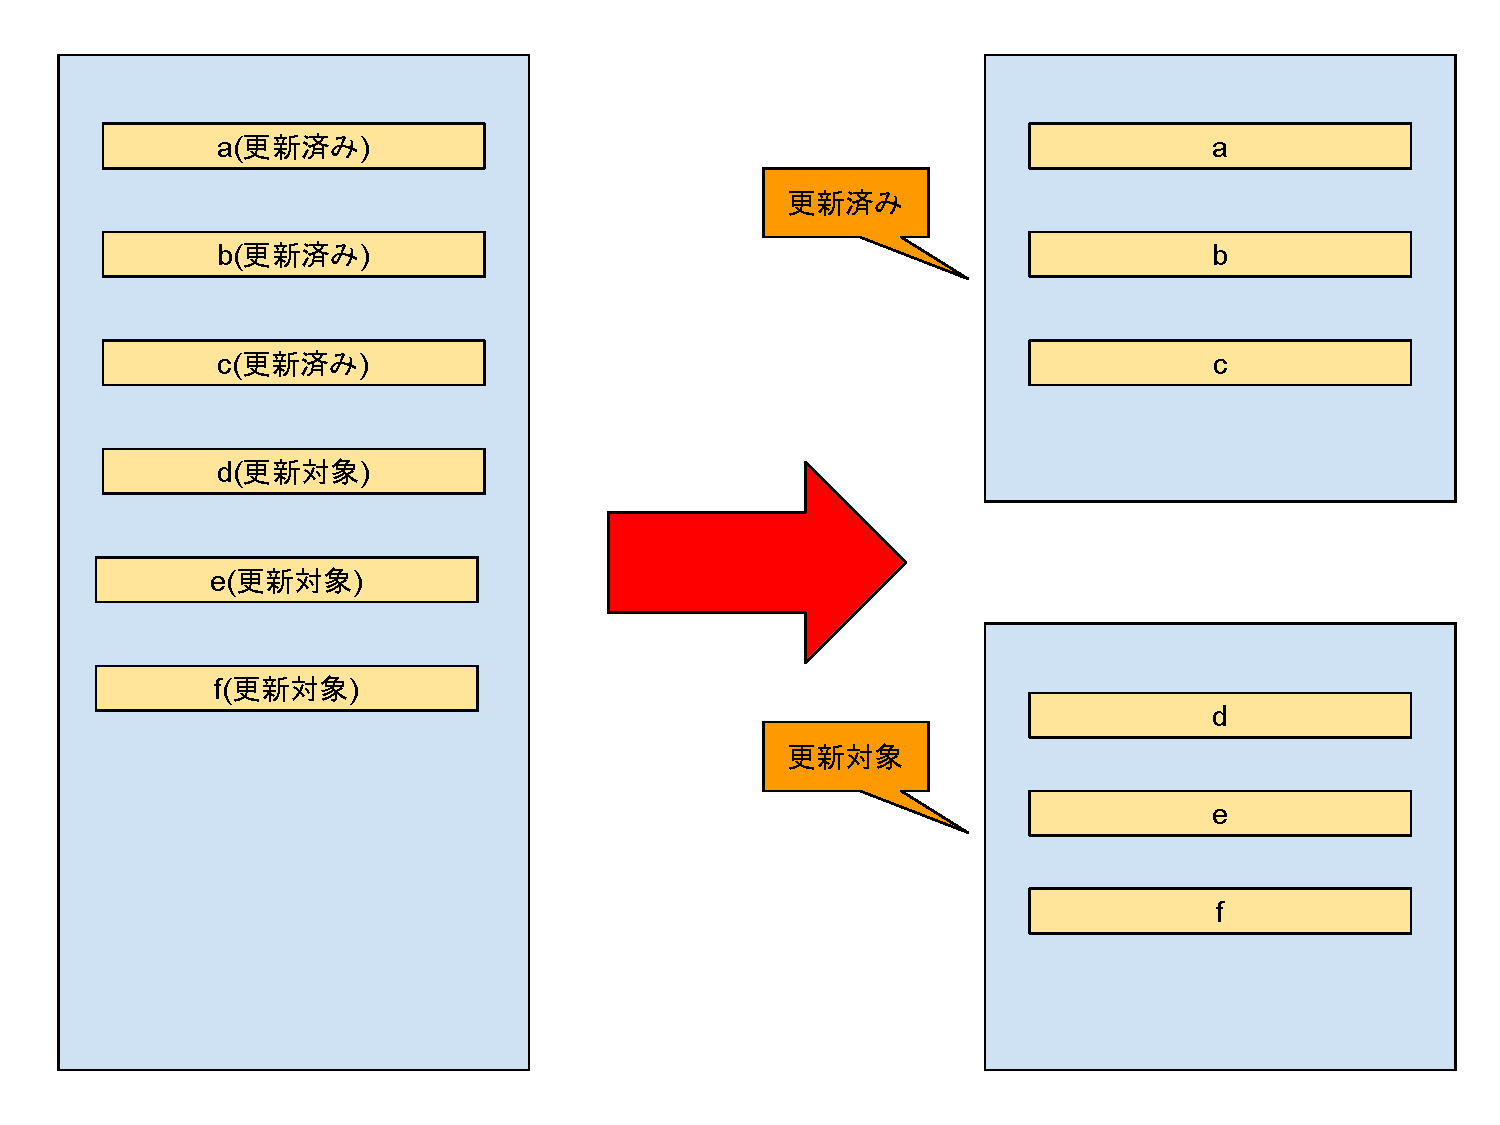
\includegraphics[width=10.0cm]{fig/fig1.pdf}
\end{figure}

完全多項式時間近似スキームによる解法は更新対象とする解のラベルと更新対象としない解のラベルを用意する
ことによってすでに更新した解を更新する無駄を削減し効率化することを目的としたアルゴリズムである.
しかし,2つのラベルを用意するため多少メモリを多く使う.
また,頂点毎の更新ではなく発見された解から順に更新されていくため,更新順序も異なる.
更新順序が異なると従来では一度解になり後の更新で削除されるはずだった解が解とならずに探索が進んでいく場合や,
従来では解にならなかったものが一度解として記憶される場合があるため探索中に更新する解の数や
削除される解の数が異なる.探索中に更新する解の数や削除される解の数が異なる
ことによって実装時間が異なる場合もある.
更新対象とするラベルと更新対象としないラベルを分けることによってすでに更新した
解を再度更新する無駄がなくなるため実装時間は短くなる.


以下に無向グラフに対するアルゴリズムを記載する.

\begin{quote}
  \textbf{記号}
  \begin{description}
    \item[$k$:] 最適化目的の数
    \item[$v \in V$,$j = 1 , \ldots , k$に対して]
    \item[$l_{jv}$:] 始点からノード$v$に到達したときに生じる
    第$j$番目の目的関数における総コスト
    \item[$e \in E$,$j = 1 , \ldots , k$に対して]
    \item[$e_{jw}$:] 辺$e$の第$j$番目の目的関数におけるコスト
    \item[$L_T$:] 更新対象とするラベル
    \item[$L_P$:] 更新対象としないラベル
  \end{description}
\end{quote}

\begin{quote}
  \textbf{アルゴリズム}
  \begin{description}
    \item[入力:] グラフ$G=(V,E)$,始点$s \in V$,最適化目的の数$k$,
    各辺の重みを返す関数$w : E \to \mathbb{R}^k$
    \item[出力:] $s$から全ての頂点への最短経路となるパレート解の集合
    \item[Step 1.] $L_T \leftarrow (s,0,\ldots,0)$,
    $L_P \leftarrow \emptyset$
    \item[Step 2.] $L_T = \{\emptyset\}$となるまで以下の操作を行う.
    \begin{description}
      \item[Step 2-1.] $L_T$の先頭にある
      $(\omega,l_{1\omega},\ldots,l_{k\omega})\in L_T$を選択する.
      \item[Step 2-2.] $L_T \leftarrow L_T \setminus
      \{ (\omega,l_{1\omega},\ldots,l_{k\omega}) \}$
      \item[Step 2-3.] 以下の条件を満たすとき,
      $L_P \leftarrow L_P \cup \{(\omega,l_{1\omega},\ldots,l_{k\omega})\}$とする.
      \begin{itemize}
        \item 任意の$(\omega^*,l_{1\omega^*},\ldots,l_{k\omega^*})\in L_P$に
        $(\omega,l_{1\omega},\ldots,l_{k\omega})$が支配されない.
        \item 任意の$(\omega^*,l_{1\omega^*},\ldots,l_{k\omega^*}) \in L_P$と
        $(\omega,l_{1\omega},\ldots,l_{k\omega})$における全ての目的関数値が同値でない.
      \end{itemize}
      \item[Step 2-4.] 頂点$\omega$に辺$e$によって接続している頂点$u$
      に対して以下の操作を行う.
      \begin{description}
        \item[Step 2-4-1.] 辺$e$の重みベクトルを
        $\vec{e} = (e_{1w},\ldots,e_{kw})$とし,
        $(\omega',l_{1\omega'},\ldots,l_{k\omega'}) \leftarrow
        (\omega',l_{1\omega}+e_{1w},\ldots,l_{k\omega}+e_{kw})$とする.
        \item[Step 2-4-2.] 以下の条件を満たすとき,
        $L_T \leftarrow L_T \cup \{(\omega',l_{1\omega'},\ldots,l_{k\omega'})\}$とする.
        \begin{itemize}
          \item 任意の$(\omega^*,l_{1\omega^*},\ldots,l_{k\omega^*})\in L_P \cup L_T$に
          $(\omega',l_{1\omega'},\ldots,l_{k\omega'})$が支配されない.
          \item 任意の$(\omega^*,l_{1\omega^*},\ldots,l_{k\omega^*}) \in L_P \cup L_T$と
          $(\omega',l_{1\omega'},\ldots,l_{k\omega'})$における全ての目的関数値が同値でない.
        \end{itemize}
        \item[Step 2-4-3.] 任意の$(\omega'',l_{1\omega''},\ldots,l_{k\omega''})\in L_T$
        に対して$(\omega',l_{1\omega'},\ldots,l_{k\omega'})$が
        $(\omega'',l_{1\omega''},\ldots,l_{k\omega''})$を支配しているとき,
        $L_T \leftarrow L_T \setminus \{(\omega'',l_{1\omega''},\ldots,l_{k\omega''})\}$とする.
      \end{description}
    \end{description}
    \item[Step 3.] 全てのパレート解を出力
  \end{description}
\end{quote}

% \begin{quote}
%   \textbf{支配}
%
%     解 $x,y$ が以下の条件を満たすとき,$x$ は $y$ を支配する.
%     \begin{itemize}
%       \item $\forall i \in \{1,\ldots,k\},f_i(x) \le f_i(y)$
%       \item $\exists i \in \{1,\ldots,k\},f_i(x) < f_i(y)$
%       \item $k$:最適化目的の数,$f$:目的関数
%     \end{itemize}
% \end{quote}

\section{ラベル付けアルゴリズムによる解法}
従来研究としてJosé Luis E. Dos Santosら\cite{Santos}に提案された
ラベル付けアルゴリズムによる解法について説明をする.
ラベル付けアルゴリズムとはいくつかのラベルを用意し,
解を分けて記憶することにより条件毎の解を参照しやすくするアルゴリズムである.
ラベル付けアルゴリズムによる解法では頂点数だけラベルを用意し,
各頂点毎の解をそれぞれのラベルに記憶していく.

\begin{figure}[htbp]
  \centering
  \caption{ラベル付けアルゴリズムによる解法と従来とのラベル比較}
  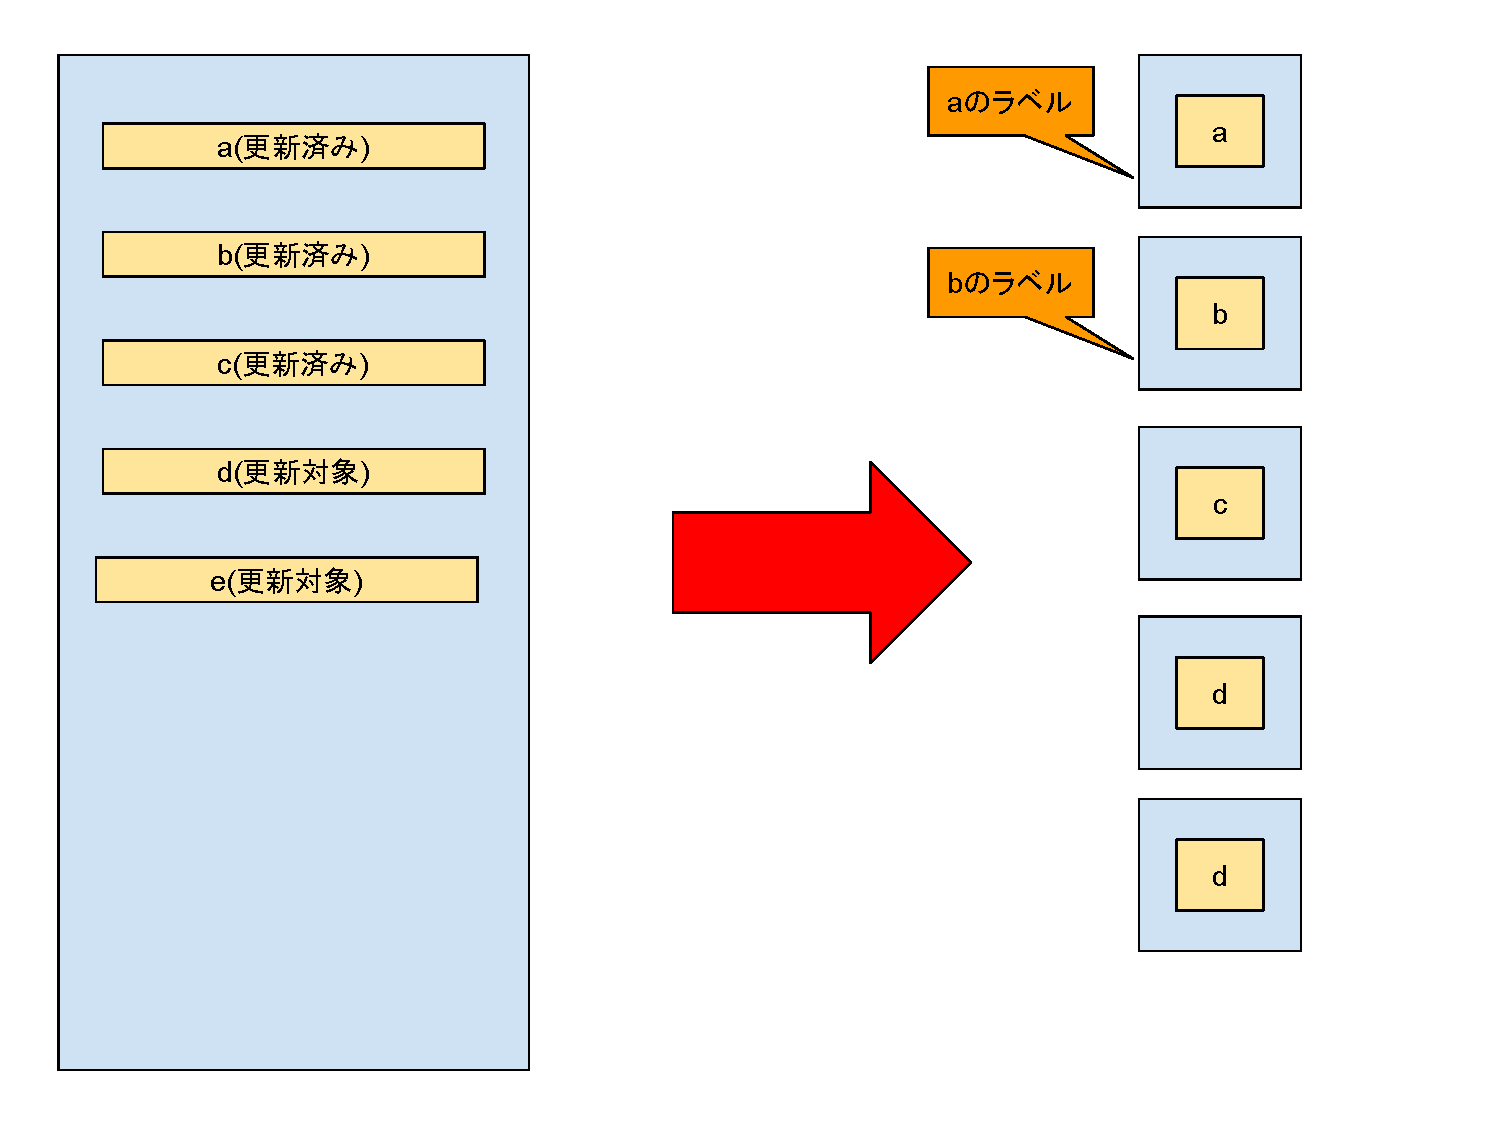
\includegraphics[width=10.0cm]{fig/fig2.pdf}
\end{figure}

従来のアルゴリズムでは1つのラベルから更新対象となる頂点に対する解を探索し
解の更新を行なっていたが,1つのラベルには全ての頂点に対する解が存在するため
多くの解に対して更新対象とするかの判定を行わなけらばならない.
ラベル付けアルゴリズムによる解法により各頂点毎の解を分けて保存しておくことが可能なので
更新対象となる頂点に対する解を選択するときに探索を行う必要がなくなり効率化になると考えられる.
ラベル付けアルゴリズムによる解法の探索方法はベルマンフォード法を改良したもので,
未更新の頂点集合を用意し,未更新の頂点がなくなるまで全辺を緩めて更新する.
ベルマンフォード法のように全ての解に対して更新を行なってしまうと無駄な更新が多く行われてしまうため
未更新の頂点集合(前回の探索によって発見された解に対する頂点集合)を
用意することによって無駄な更新を削減している.


以下に無向グラフに対するアルゴリズムを記載する.

\begin{quote}
  \textbf{記号}
  \begin{description}
    \item[$k$:] 最適化目的の数
    \item[$v \in V$に対して]
    \item[$L_v$:] 頂点$v$に対するラベル
    \item[$v \in V$,$j = 1 , \ldots , k$に対して]
    \item[$l_{jv}$:] 始点からノード$v$に到達したときに生じる
    第$j$番目の目的関数における総コスト
    \item[$e \in E$,$j = 1 , \ldots , k$に対して]
    \item[$e_{jw}$:] 辺$e$の第$j$番目の目的関数におけるコスト
    \item[$X$:] 更新対象とする頂点集合
  \end{description}
\end{quote}

\begin{quote}
  \textbf{アルゴリズム}
  \begin{description}
    \item[入力:] グラフ$G=(V,E)$,始点$s \in V$,最適化目的の数$k$,
    各辺の重みを返す関数$w : E \to \mathbb{R}^k$
    \item[出力:] $s$から全ての頂点への最短経路となるパレート解の集合
    \item[Step 1.] $\forall v \in V , L_v \leftarrow \emptyset$,
    $L_s \leftarrow (s,0,\ldots,0)$,$X \leftarrow s$
    \item[Step 2.] $X = \{\emptyset\}$となるまで以下の操作を行う.
    \begin{description}
      \item[Step 2-1.] $v \in X$となる頂点$v$を選択する.
      \item[Step 2-2.] $X \leftarrow X \setminus \{ v \}$
      \item[Step 2-3.] $e = {e \in E \mid v,u \in e}$となる
      $e$に対して以下の操作を行う.
      \begin{description}
        \item[Step 2-3-1.] 頂点$v$に対する全てのpath
        $(v',l_{1v'},\ldots,l_{kv'}) \in L_v$に対して以下の操作を行う.
        \begin{description}
          \item[Step 2-3-1-1.] 辺$e$の重みベクトルを
          $\vec{e} = (e_{1w},\ldots,e_{kw})$とし,
          $(u',l_{1u'},\ldots,l_{ku'}) \leftarrow
          (u',l_{1v}+e_{1w},\ldots,l_{kv}+e_{kw})$とする.
          \item[Step 2-3-1-2.] 以下の条件を満たすとき,
          $L_u \leftarrow L_u \cup \{(u',l_{1u'},\ldots,l_{ku'})\}$,
          $X \leftarrow X \cup \{ u\}$とする.
          \begin{itemize}
            \item 任意の$(u^*,l_{1u^*},\ldots,l_{ku^*})\in L_u$に
            $(u',l_{1u'},\ldots,l_{ku'})$が支配されない.
            \item 任意の$(u^*,l_{1u^*},\ldots,l_{ku^*}) \in L_u$と
            $(u',l_{1u'},\ldots,l_{ku'})$における全ての目的関数値が同値でない.
          \end{itemize}
          \item[Step 2-3-1-3.] 任意の$(u'',l_{1u''},\ldots,l_{ku''})\in L_u$
          に対して$(u',l_{1u'},\ldots,l_{ku'})$が
          $(u'',l_{1u''},\ldots,l_{ku''})$を支配しているとき,
          $L_u \leftarrow L_u \setminus \{(u'',l_{1u''},\ldots,l_{ku''})\}$とする.
        \end{description}
      \end{description}
    \end{description}
    \item[Step 3.] 全てのパレート解を出力
  \end{description}
\end{quote}


\chapter{解法の提案と実験的評価}
この章では,多目的最短経路問題についての分析を行い解法の考察をする.
その後,提案解法の紹介と実装における工夫,本研究に対する成果を述べる.

\section{問題の分析}
本研究では多目的単一始点最短経路問題を扱う.
多目的単一始点最短経路問題とは特定の1つのノードから他の全ノードとの間の最短経路問題であり,
入力と出力は以下のようになる.
\begin{itemize}
  \item[入力:]重み付きグラフ,始点$s$,最適化目的の数$k$
  \item[出力:]$s$から全頂点へのパレート最適解となる経路の集合
\end{itemize}

\begin{description}
  \item[パレート最適解の集合の数に対する問題の難しさ]
\end{description}

一般的に多目的最適化問題は出力となるパレート最適解の数に比例して解くことが難しくなる.
これは解の探索をするとともに,パレート最適解であるかどうかの判定のために既知の解と比較をするためである.
単目的最短経路問題の場合,1つの頂点に1つの解しか存在しないため既知の解との比較は1回である.
しかし,多目的最適問題の場合,1つの頂点に対して始点と終点を結ぶpathの本数分の解が存在する.
任意の頂点$v \in V$を選択する.頂点集合$V$から始点$s$と$v$を除いた頂点集合を$V'=V \setminus \{s\}$とする.
pathは始点から終点への通過する頂点の順番で表されるため,通過する頂点の集合の並び替えの数だけ存在する.
$s$から$v$へのpathの数は$V'$から$i$個の頂点を選択し並び変えた数だけ存在する.
頂点数を$|N|=n$とすると$V'$の要素数は$|V'|=n-2$なので,
$\displaystyle \sum_{i=0}^{n-2} {}_{(n-2)}C_i i!$で表される.
よって,既知の解との比較は最大で$\displaystyle \sum_{i=0}^{n-2} {}_{(n-2)}C_i i!$回である.
既知の解との比較は,単目的最短経路問題では1回であり,
多目的最適問題では最大で$\displaystyle \sum_{i=0}^{n-2} {}_{(n-2)}C_i i!$回であるため
パレート最適解の数に比例して解くことが難しくなる.
パレート最適解の数に比例して解くことが難しくなることを照明したため,
それぞれのインスタンスに対してパレート最適解の数がどのように変化するか分析する.

\begin{description}
  \item[頂点数に対する問題の難しさ]
\end{description}

パレート最適解の数が問題の難しさに直結することを示した.頂点数に対する問題の難しさを分析するために,
入力の頂点数$|V|=n$によりパレート最適解の数がどのように変化するか分析する.
頂点数とパレート最適解の集合の数の関係を分析するためにその他の入力は
辺の重みベクトルの値がランダムであり,重みの範囲が十分に大きい完全グラフとする.
多目的最短経路問題の場合,解は始点から各頂点へのpathの本数分存在する.
頂点集合$V$から始点$s$を除いた頂点集合を$V'=V \setminus \{s\}$とする.
pathは始点から終点への通過する頂点の順番で表されるため,通過する頂点の集合の並び替えの数だけ存在する.
完全グラフにおいて始点から各頂点へのpathの合計は$V'$から$i$個の頂点を選択し並び変えた数だけ存在する.
$V'$の要素数は$|V'|=n-1$なので,$\displaystyle \sum_{i=0}^{n-1} {}_{(n-1)}C_i i!$で表される.
以上より,頂点数が大きくなるとパレート最適解の数は指数的に増えるため,頂点数が大きくなると
問題は難しくなる.

\begin{description}
  \item[重みの範囲に対する問題の難しさ]
\end{description}

パレート最適解の数が問題の難しさに直結することを示した.重みの範囲に対する問題の難しさを分析するために,
全ての重みが非負数である完全グラフにおいて重みの範囲によりパレート最適解の数がどのように変化するか分析する.
重みの範囲によりパレート最適解の集合の数の関係を分析するためにその他の入力は
辺の重みベクトルの値がランダムであり,頂点数が十分に大きい完全グラフとする.
始点$s$から終点$t$への最短経路を求める.頂点$v$を経由した$s$から$t$への経路を$(s,v,t)$と表す.
非負数であるグラフにおいて,経由する頂点数が多くなるほど各目的関数の値は大きくなるため,
経路$(s,t)$が経路$(s,v,t)$を支配する確率は高くなる.
また,経路$(s,t)$が$i$個の頂点を経由する経路$(s,v_1,\ldots,v_i,t)$を支配する確率も高くなる.
ここで,重みの範囲が広くなると経路$(s,v,t)$が解となる確率は高くなるため解の数は多くなると予想される.
経由する頂点1つの場合,重みの範囲に対して解になる確率が高くなることを示したが,経由する頂点数が増加した場合でも
同じく重みの範囲に対して解になる確率が高くなると予想されるため全体の解の数はさらに多くなると予想される.
経由する頂点数が増えるほど解になる確率が低くなっていくが,重みの範囲が広くなると解の確率は上がるため,
一定の範囲で2つの確率が相殺しあうため,重みの範囲が一定の値を越えると解は増えなくなる.
以上より,重みの範囲が広くなると最適解の数は増えるため,重みの範囲が広くなると問題は難しくなる.


証明:
最適化目的の数が2$(f_1,f_2)$,重みの範囲が1であるグラフを考える.任意の2頂点間の目的関数の組み合わせは
$f_1$が$0,1$の2通り,$f_2$が$0,1$の2通りなので$2 \times 2$の4通りである.
経路$(s,t)$が経路$(s,v,t)$の組み合わせは経路3本の組み合わせなので$4^3 = 64$通り.
ここで,経路$(s,t)$が経路$(s,v,t)$を支配するまたは同値である組み合わせを考える.
上記の組み合わせが成立するためには以下が成り立たなければならない.経路$(s,t)$の各目的関数$f_{st1},f_{st2}$,
経路$(s,v)$の各目的関数$f_{sv1},f_{sv2}$,経路$(v,t)$の各目的関数$f_{vt1},f_{vt2}$において
$f_{st1}>f_{sv1}+f_{vt1}$または$f_{st2}>f_{sv2}+f_{vt2}$.これは$f_{st1}=1$かつ$f_{sv1}+f_{vt1}=0$,
$f_{st2}=1$かつ$f_{sv2}+f_{vt2}=0$なので$2^3+2^3-1=15$通り.
よって経路$(s,v,t)$が解となる確率は$15/64=0.234$である.
最適化目的の数が2$(f_1,f_2)$,重みの範囲が2であるグラフを考える.任意の2頂点間の目的関数の組み合わせは
$f_1$が$0,1,2$の2通り,$f_2$が$0,1,2$の3通りなので$3 \times 3$の9通りである.
経路$(s,t)$が経路$(s,v,t)$の組み合わせは経路3本の組み合わせなので$9^3 = 729$通り.
ここで,経路$(s,t)$が経路$(s,v,t)$を支配するまたは同値である組み合わせを考える.
上記の組み合わせが成立するためには以下が成り立たなければならない.経路$(s,t)$の各目的関数$f_{st1},f_{st2}$,
経路$(s,v)$の各目的関数$f_{sv1},f_{sv2}$,経路$(v,t)$の各目的関数$f_{vt1},f_{vt2}$において
$f_{st1}>f_{sv1}+f_{vt1}$または$f_{st2}>f_{sv2}+f_{vt2}$.
これは$(3^3+3^3-1)+(3 \times 3^3 + 3 \times 3^3 - 3)=53+159=212$通り.
よって経路$(s,v,t)$が解となる確率は$212/729=0.291$である.
以上より,重みの範囲が広くなると経路$(s,v,t)$が解となる確率は高くなる.

\begin{description}
  \item[最適化目的の数に対する問題の難しさ]
\end{description}

パレート最適解の数が問題の難しさに直結することを示した.最適化目的の数に対する問題の難しさを分析するために,
全ての重みが非負数である完全グラフにおいて最適化目的の数によりパレート最適解の数がどのように変化するか分析する.
最適化目的の数によりパレート最適解の集合の数の関係を分析するためにその他の入力は
辺の重みベクトルの値がランダムかつ重みの範囲が十分に大きい値であり,頂点数が十分に大きい完全グラフとする.
始点$s$から終点$t$への最短経路を求める.頂点$v$を経由した$s$から$t$への経路を$(s,v,t)$と表す.
非負数であるグラフにおいて,経由する頂点数が多くなるほど各目的関数の値は大きくなるため,
経路$(s,t)$が経路$(s,v,t)$を支配する確率は高くなる.
また,経路$(s,t)$が$i$個の頂点を経由する経路$(s,v_1,\ldots,v_i,t)$を支配する確率も高くなる.
最適化目的の数が2の場合と3の場合を比較する.$(s,t)$の各目的関数を$f_{st1},f_{st2},f_{st3}$,
$(s,v,t)$の各目的関数を$f_{svt1},f_{svt2},f_{svt3}$とする.
経路$(s,v,t)$が解となるためには1つでも目的関数が$(s,t)$より低ければ良い.
つまり,$\exists i ,f_{svti}<f_{sti}$が成り立てば良い.
最適化目的の数が2の場合$i$の選択肢は2つだが,最適化目的の数が3の場合$i$の選択肢は3つとなり
$\exists i ,f_{svti}<f_{sti}$が成り立つ可能性が高くなる.
よって,最適化目的の数が増えると頂点を1つ経由した経路が解となる確率が高くなる.
経由する頂点数が増えた場合でも同じことが言えるので全体の解の数はさらに増えると予想される.
以上より,最適化目的の数が増えると最適解の数は増えるため,最適化目的の数が増えると問題は難しくなる.

\begin{description}
  \item[辺の本数に対する問題の難しさ]
\end{description}

パレート最適解の数が問題の難しさに直結することを示した.辺の本数に対する問題の難しさを分析するために,
全ての重みが非負数であるグラフにおいて辺の本数によりパレート最適解の数がどのように変化するか分析する.
辺の本数によりパレート最適解の集合の数の関係を分析するためにその他の入力は,最適化目的の数が$k$,
辺の重みベクトルの値がランダム,重みの範囲が十分に大きい,頂点数が十分に大きいグラフとする.
始点$s$から終点$t$への最短経路を求める.頂点$v$を経由した$s$から$t$への経路を$(s,v,t)$と表す.
完全グラフの場合,頂点を1つ経由する経路は始点と終点を除いた頂点集合から1頂点を選択した経路なので
$n-2$通り存在する.グラフ上の$s$と$t$を除いた頂点集合の任意の頂点$v'$について,$s$と$v'$
を結ぶ辺が存在しない又は$v'$と$t$を結ぶ辺が存在しないとき,頂点$v'$を通る経路$(s,v,t)$は存在しない.
また,頂点$u$と頂点$u'$を結ぶ辺が存在しないとき,$(s,\ldots, u, u', \ldots , t$となるような経路は存在しない.
このように辺の本数が少なくなると,グラフ上の経路は少なくなるため解の候補となる経路の数が減少する.
よって,全体の解の数は少なくなる.単一始点最短経路問題において,始点$s$を中心としたスターグラフ内の
解となり得る経路は$n-1$本存在する.単一始点最短経路問題において,完全グラフ内の解となり得る経路は
$\displaystyle \sum_{i=0}^{n-1} {}_{(n-1)}C_i i!$本存在する.
以上より,辺の本数が増えると最適解の数は増えるため,辺の本数が増えると問題は難しくなる.

\begin{description}
  \item[各目的関数間の相関に対する問題の難しさ]
\end{description}

パレート最適解の数が問題の難しさに直結することを示した.各目的関数間の相関に対する問題の難しさを分析するために,
全ての重みが非負数である完全グラフにおいて各目的関数間の相関によりパレート最適解の数がどのように変化するか分析する.
各目的関数間の相関によりパレート最適解の集合の数の関係を分析するためにその他の入力は,最適化目的の数が3,
辺の重みベクトルの値がランダム,重みの範囲が十分に大きい,頂点数が十分に大きい完全グラフとする.
相関は−1〜1で表され,−1に近いほど負の相関があり,0に近いほど相関がなく,1に近いほど正の相関があるという.
以下では頂点に入ってくる辺の重みベクトルに対する相関と頂点から出ていく辺の重みベクトルに対する相関に対する分析を行う.

頂点に入ってくる辺の重みベクトルに対する相関に対する分析.
最適化目的の数3のため,各目的関数を$(f_1,f_2,f_3)$とし,任意の辺$e \in E$における重みベクトルを
$\vec{e}=(e(f_1),e(f_2),e(f_3))$とする.終点が頂点$u$である辺(頂点$u$に入ってくる辺)の集合を$E_u$とする.
頂点に入ってくる辺の重みベクトルに対する相関とは3つある.$\forall E_v , v \in V$に対する相関であり,それぞれ
$\{f_1,f_2\}$間の相関$c_{12}$,$\{f_2,f_3\}$間の相関$c_{23}$,$\{f_1,f_3\}$間の相関$c_{13}$である.
$c_{12}=1$のとき,任意の辺$x,v\in E$に対して,$x(f_1)=x(f_2)\times l$のとき$y(f_1)=y(f_2)\times l$が成り立つ.
つまり,$c_{12}=1$のとき,任意の辺$x,v\in E$に対して,$x(f_1)<x(f_2) \land y(f_1)<y(f_2)$または
$x(f_1)=x(f_2) \land y(f_1)=y(f_2)$または$x(f_1)>x(f_2) \land y(f_1)>y(f_2)$が成り立つ.
$c_{12}=1,c_{23}=1$のとき$c_{13}=1$である.このとき,任意の辺$e \ inE$を$\vec{e}=(e(f_1),e(f_2),e(f_3))$とすると
$\forall e'\in E,\vec{e'} = l\times(e(f_1),e(f_2),e(f_3))$が成り立つため各頂点に対する解の数はそれぞれ1となり,
全体の解の数は$|N|$となる.また,各目的関数間の相関が強ければ強いほど頂点$u\in V$における$s$からの経路$u'_{s}$と
$u''_{s}$に対して,支配関係($u'_{s}$が$u''_{s}$を支配するまたは$u''_{s}$が$u'_{s}$を支配する)が成り立つ可能性が
高いため全体の解の数は少なくなる.
以上より,頂点に入ってくる辺の重みベクトルに対する相関が弱いと最適解の数は増えるため,
頂点に入ってくる辺の重みベクトルに対する相関が弱いと問題は難しくなる.


頂点から出ていく辺の重みベクトルに対する相関に対する分析.
最適化目的の数3のため,各目的関数を$(f_1,f_2,f_3)$とし,任意の辺$e \in E$における重みベクトルを
$\vec{e}=(e(f_1),e(f_2),e(f_3))$とする.始点が頂点$u$である辺(頂点$u$から出ていく辺)の集合を$E_u$とする.
頂点から出ていく辺の重みベクトルに対する相関とは3つある.$\forall E_v , v \in V$に対する相関であり,それぞれ
$\{f_1,f_2\}$間の相関$c_{12}$,$\{f_2,f_3\}$間の相関$c_{23}$,$\{f_1,f_3\}$間の相関$c_{13}$である.
$c_{12}=1$のとき,任意の辺$x,v\in E$に対して,$x(f_1)=x(f_2)\times l$のとき$y(f_1)=y(f_2)\times l$が成り立つ.
つまり,$c_{12}=1$のとき,任意の辺$x,v\in E$に対して,$x(f_1)<x(f_2) \land y(f_1)<y(f_2)$または
$x(f_1)=x(f_2) \land y(f_1)=y(f_2)$または$x(f_1)>x(f_2) \land y(f_1)>y(f_2)$が成り立つ.
$c_{12}=1,c_{23}=1$のとき$c_{13}=1$である.このとき,任意の辺$e \ inE$を$\vec{e}=(e(f_1),e(f_2),e(f_3))$とすると
$\forall e'\in E,\vec{e'} = l\times(e(f_1),e(f_2),e(f_3))$が成り立つため各頂点に対する解の数はそれぞれ1となり,
全体の解の数は$|N|$となる.また,各目的関数間の相関が強ければ強いほど頂点$u\in V$における$s$からの経路$u'_{s}$と
$u''_{s}$に対して,支配関係($u'_{s}$が$u''_{s}$を支配するまたは$u''_{s}$が$u'_{s}$を支配する)が成り立つ可能性が
高いため全体の解の数は少なくなる.
以上より,頂点から出ていく辺の重みベクトルに対する相関が弱いと最適解の数は増えるため,
頂点から出ていく辺の重みベクトルに対する相関が弱いと問題は難しくなる.


\begin{description}
  \item[多目的最短経路問題に対する単目的最短経路問題アルゴリズムの実装]
\end{description}

入力が,頂点集合$V$($|V|=n$),最適化目的の数が$k$,
辺の重みベクトルの値がランダム(相関がない),重みの範囲が十分に大きい,完全グラフとする.
本研究では重みがランダム(異なる)単一始点最短経路を扱うため,単一目的最短経路問題での解法は
ダイクストラ法とベルマンフォード法である.(重みが決まった値でないため幅優先探索は扱えない.
全点対最短経路でないためワーシャルフロイド法は効率的でない.)
多目的最短経路問題に対するダイクストラ法とベルマンフォード法の適用を実装し,それぞれの問題点と活用方法を分析する.

ダイクストラ法の適用.ダイクストラ法はすでに探索済みのノードの中で重みが最小のノードを
求め,更新対象として探索していくアルゴリズムである.全ての重みが非負数の場合,探索したノードの中で重みが最小のものは
その後の探索で更新されることはないので重みが決定する.多目的最短経路問題にダイクストラ法を適用すると
すでに探索済みのpathの中で重みが最小のpathを求め,更新対象として探索していく.
全ての重みが非負数の場合,探索したpathの中で重みが最小のものはその後の探索で支配されることはないので解として決定する.
ダイクストラ法の問題点は重みが最小であるpathの探索であり,理由は2つある.1つ目の理由は多目的最適化問題においてpathは
複数の目的関数を所持しているため最小である基準が明確でないことである.単目的最短経路問題では目的関数が1つ
のためその目的関数が最小のpath(頂点)を選択すれば良い.目的関数が複数である多目的最短経路問題では,
各目的関数に対して評価値をもうけ優先順位をつける方法(例:目的関数が$f_1,f_2,f_3$のとき
$f_2 \rightarrow f_1 \rightarrow f_3 $という優先順位をつける)や1つの目的関数として計算する方法
(例:目的関数が$f_1,f_2,f_3$のとき$f_x = f_1 + f_2 \times 2 + f_3 \times 4$という目的関数を計算する)
が考えられる.もう1つの問題は重みが最小であるpath(更新対象)の探索するために多くの比較が必要となることである.
単目的最短経路問題の場合選択肢となるpath(頂点)は頂点数分なので最大で$|N|$つあるが,多目的最短経路の場合
選択肢となるpathは1頂点に対して複数存在するため最大で$\displaystyle \sum_{i=0}^{n-1} {}_{(n-1)}C_i i!$
つとなる.探索のたびにこれらのpathの中から1つのpathを選択するには毎回それぞれの値を比較して
対象となるpathを求めなければならないため膨大な計算時間がかかる.これらの問題に対して
pathが発見されるたびに更新順のリストに保存していく方法があるが,リストへの保存に対しても
多くの計算時間がかかるため問題は難しいままである.

ベルマンフォード法の適用.ベルマンフォード法は頂点数を $|V|$ とした時,全辺を緩めることを単に $|V|-1$ 回繰り返すアルゴリズムである.
多目的最短経路問題にベルマンフォード法を適用すると,単目的最短経路問題と同じように頂点数を $|V|$ とした時,
全辺を緩めることを単に $|V|-1$ 回繰り返す.ダイクストラ法と違い,更新対象を探索する操作がないため
ダイクストラ法のボトルネックとなっていた目的関数が最小のpath(頂点)を選択するための比較や計算をしなくて済む.
しかし,全辺を緩める操作のときにすでに更新したpathまで更新対象としてしまうため無駄が生じてしまう.
単目的最短経路問題の場合,各頂点に最大で1つの解(path)が存在するため1回の全辺を緩める操作で更新対象となるのは
最大で頂点数である$|V|$である.一方,多目的最短経路問題では各頂点に最大で始点からのpathの本数分
(完全グラフの場合,存在する始点からのpathの本数は$\displaystyle \sum_{i=0}^{n-2} {}_{(n-2)}C_i i!$本)
存在する.また,1回の全辺を緩める操作で更新対象となるのは最大で$\displaystyle \sum_{i=0}^{n-1} {}_{(n-1)}C_i i!$つとなる.
そのため,全辺を緩めることを単に $|V|-1$ 回繰り返してしまうと膨大な計算時間がかかってしまう.

\section{非負数の問題に対する解法の提案}
非負数である多目的最短経路問題における解法を提案する.

\subsection{提案解法1}
多目的最短経路問題に対する単目的最短経路問題アルゴリズムの実装で述べたようにダイクストラ法とベルマンフォード法
にはそれぞれボトルネックがあるため改良が必要である.ダイクストラ法のボトルネックである更新対象の探索
はヒープを用いた方法やpathが発見されるたびに更新順のリストに保存していく方法があるが目的関数が増えていくと
これらの操作時間にも計算時間がかかってしまうため現実的でない.一方,ベルマンフォード法は改善によって
ボトルネックを解決できる.そのため,最適な解法を得るためにベルマンフォード法の改善をしていく.

まず,ベルマンフォード法のボトルネックである全辺を緩めることを単に$|V|-1$ 回繰り返してしまうと膨大な計算時間がかかってしまう
という問題と,1回の全辺を緩める操作で更新対象となるのは最大で$\displaystyle \sum_{i=0}^{n-1} {}_{(n-1)}C_i i!$つとなる問題を
解決した解法を以下に記載する.


\begin{quote}
  \textbf{記号}
  \begin{description}
    \item[$k$:] 最適化目的の数
    \item[$L$:] 解となるラベル
    \item[$X$:] 更新対象とする頂点集合
    \item[$v \in V$,$j = 1 , \ldots , k$に対して]
    \item[$l_{jv}$:] 始点からノード$v$に到達したときに生じる
    第$j$番目の目的関数における総コスト
    \item[$e \in E$,$j = 1 , \ldots , k$に対して]
    \item[$e_{jw}$:] 辺$e$の第$j$番目の目的関数におけるコスト
  \end{description}
\end{quote}

\begin{quote}
  \textbf{アルゴリズム}
  \begin{description}
    \item[入力:] グラフ$G=(V,E)$,始点$s \in V$,最適化目的の数$k$,
    各辺の重みを返す関数$w : E \to \mathbb{R}^k$
    \item[出力:] $s$から全ての頂点への最短経路となるパレート解の集合
    \item[Step 1.] $\forall v \in V , L_v \leftarrow \emptyset$,
    $L_s \leftarrow (s,0,\ldots,0)$,$X \leftarrow s$
    \item[Step 2.] $X = \{\emptyset\}$となるまで以下の操作を行う.
    \begin{description}
      \item[Step 2-1.] $v \in X$となる頂点$v$を選択する.
      \item[Step 2-2.] $X \leftarrow X \setminus \{ v \}$
      \item[Step 2-3.] $e = {e \in E \mid v,u \in e}$となる
      $e$に対して以下の操作を行う.
      \begin{description}
        \item[Step 2-3-1.] 頂点$v$に対する全てのpath
        $(v',l_{1v'},\ldots,l_{kv'}) \in L,v=v'$に対して以下の操作を行う.
        \begin{description}
          \item[Step 2-3-1-1.] 辺$e$の重みベクトルを
          $\vec{e} = (e_{1w},\ldots,e_{kw})$とし,
          $(u',l_{1u'},\ldots,l_{ku'}) \leftarrow
          (u',l_{1v}+e_{1w},\ldots,l_{kv}+e_{kw})$とする.
          \item[Step 2-3-1-2.] 以下の条件を満たすとき,
          $L \leftarrow L \cup \{(u',l_{1u'},\ldots,l_{ku'})\}$,
          $X \leftarrow X \cup \{ u\}$とする.
          \begin{itemize}
            \item 任意の$(u^*,l_{1u^*},\ldots,l_{ku^*})\in L,u=u^*$に
            $(u',l_{1u'},\ldots,l_{ku'})$が支配されない.
            \item 任意の$(u^*,l_{1u^*},\ldots,l_{ku^*}) \in L,u=u^*$と
            $(u',l_{1u'},\ldots,l_{ku'})$における全ての目的関数値が同値でない.
          \end{itemize}
          \item[Step 2-3-1-3.] 任意の$(u'',l_{1u''},\ldots,l_{ku''})\in Lu=u''$
          に対して$(u',l_{1u'},\ldots,l_{ku'})$が
          $(u'',l_{1u''},\ldots,l_{ku''})$を支配しているとき,
          $L \leftarrow L \setminus \{(u'',l_{1u''},\ldots,l_{ku''})\}$とする.
        \end{description}
      \end{description}
    \end{description}
    \item[Step 3.] 全てのパレート解を出力
  \end{description}
\end{quote}


上記の解法は更新によって新たな解を得た頂点を更新対象となる頂点集合に加えることによって,更新しなくて良い頂点を
更新せずに済む.これにより,1回の全辺を緩める操作で更新対象となるのは最大で
$\displaystyle \sum_{i=0}^{n-1} {}_{(n-1)}C_i i!$つとなる問題を解決した.
また,更新対象とする頂点が存在しなくなった時点で探索が終了するため全辺を緩めることを単に$|V|-1$ 回
繰り返してしまうと膨大な計算時間がかかってしまうという問題を解決した.
しかし,この解法にはまだ改善点がいくつか存在するためそれらの改善をしていく.
この解法の問題点は2つある.1つ目はすでに更新済みであるpathを更新対象にしているために無駄な更新が行われている点である.
頂点に対する解であるpathは複数存在している.頂点$v$に対してすでに更新済みであるpathを$a,b$とし,他の頂点の更新により
新しく得られたpathを$c,d$とすると,次に頂点$v$の更新を行うときpath$c,d$のみを更新対象とすれば良い.
上記の解法では頂点に対するpath$a,b,c,d$すべてが更新対象となってしまうためpath$a,b$の無駄な更新が行われてしまう.
2つ目はパレート最適解の判定の際に比較対象となるpathを探索するのに多くの計算時間がかかってしまう点である.
上記の解法では解となるpathを保存するラベルが1つのため比較対象となるpathを選択するためにすでに求めてある
path全てを探索する必要がある.全てのpathは最大で$\displaystyle \sum_{i=0}^{n-1} {}_{(n-1)}C_i i!$つ
存在し,比較対象とするpathは最大で$\displaystyle \sum_{i=0}^{n-2} {}_{(n-2)}C_i i!$のため選択のための
探索に膨大な計算時間がかかってしまう.

\begin{figure}[htbp]
  \centering
  \caption{ベルマンフォード改良解法と従来のラベル比較}
  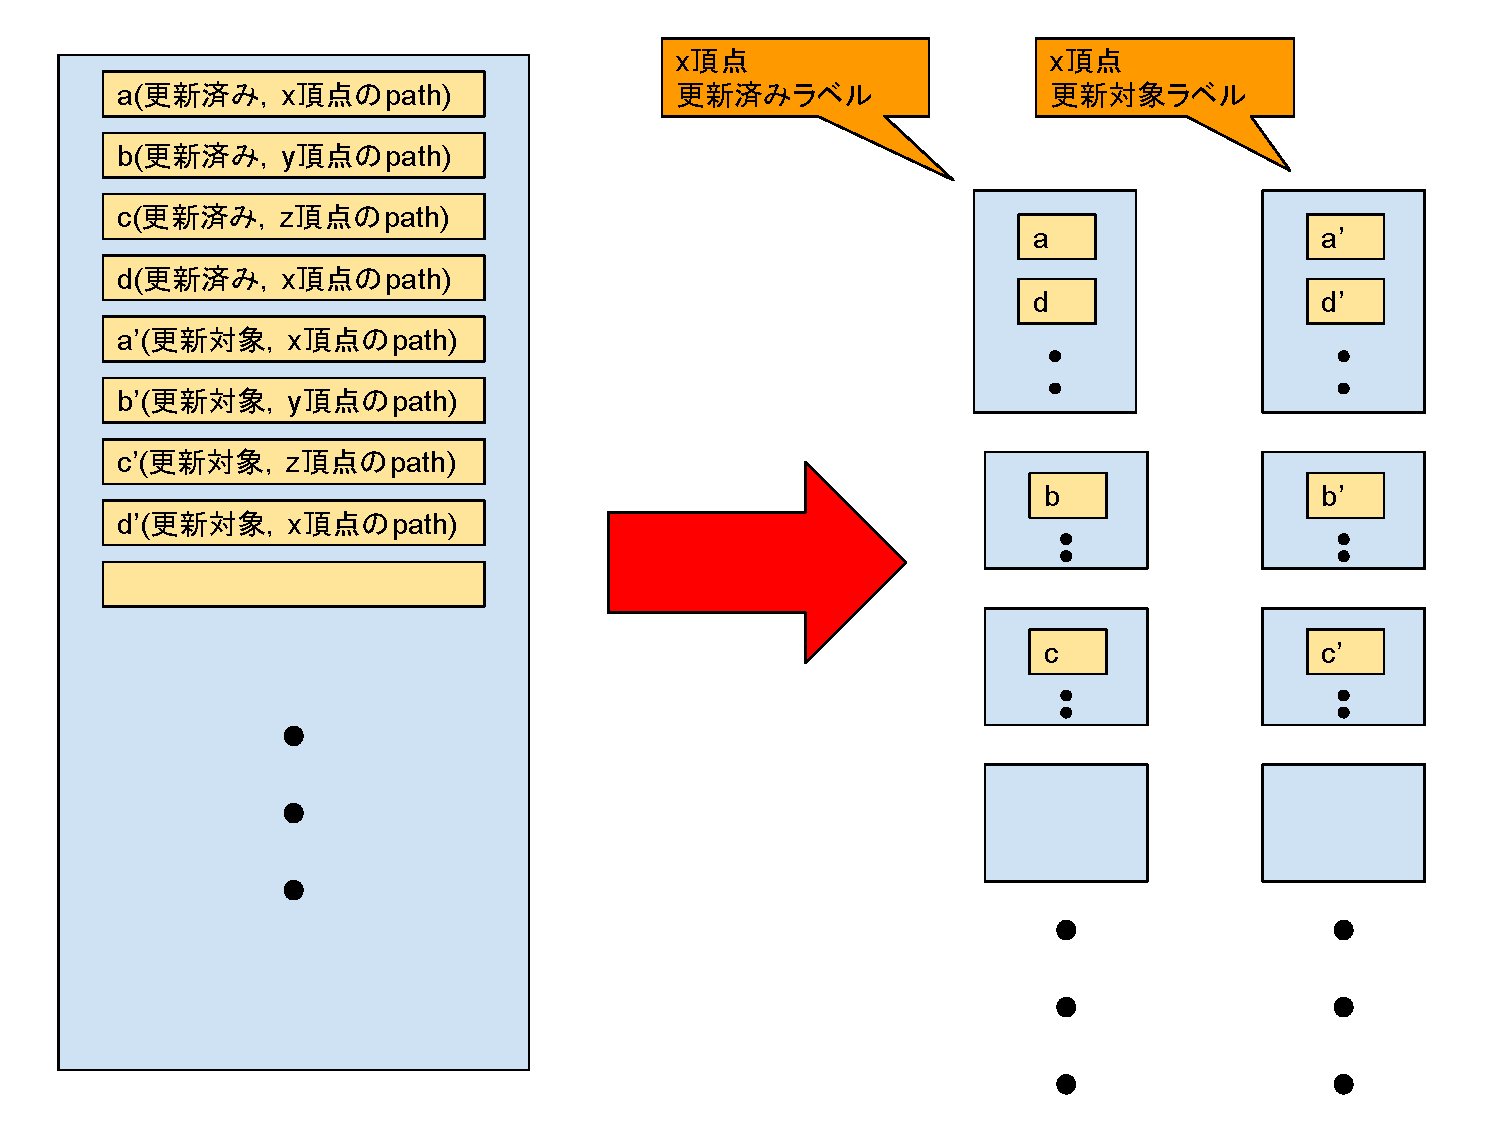
\includegraphics[width=10.0cm]{fig/fig3.pdf}
\end{figure}

上記の解法の問題点を解決するために,従来研究で提案された完全多項式時間近似スキームによる解法と
ラベル付けアルゴリズムによる解法を組み合わせ改良を加える.
まず,完全多項式時間近似スキームによる解法で提案されたように,更新対象とする解のラベルと更新対象としない解のラベルを用意する
ことによって無駄な更新を削減し効率化する.これによりpath$c,d$のみを更新対象とすることができるため
path$a,b$の無駄な更新を行わずにすむ.つぎに,ラベル付けアルゴリズムによる解法で提案されたように
頂点数だけラベルを用意し,各頂点毎の解をそれぞれのラベルに記憶していく.
従来のアルゴリズムでは1つのラベルから更新対象となる頂点に対する解を探索し
解の更新を行なっていたが,1つのラベルには全ての頂点に対する解が存在するため
多くの解に対して更新対象とするかの判定を行わなけらばならない.
ラベル付けアルゴリズムによる解法により各頂点毎の解を分けて保存しておくことが可能なので
更新対象となる頂点に対する解を選択するときに探索を行う必要がなくなり効率化になると考えられる.


\begin{figure}[htbp]
  \centering
  \caption{ラベルの統合(提案解法1のラベル)}
  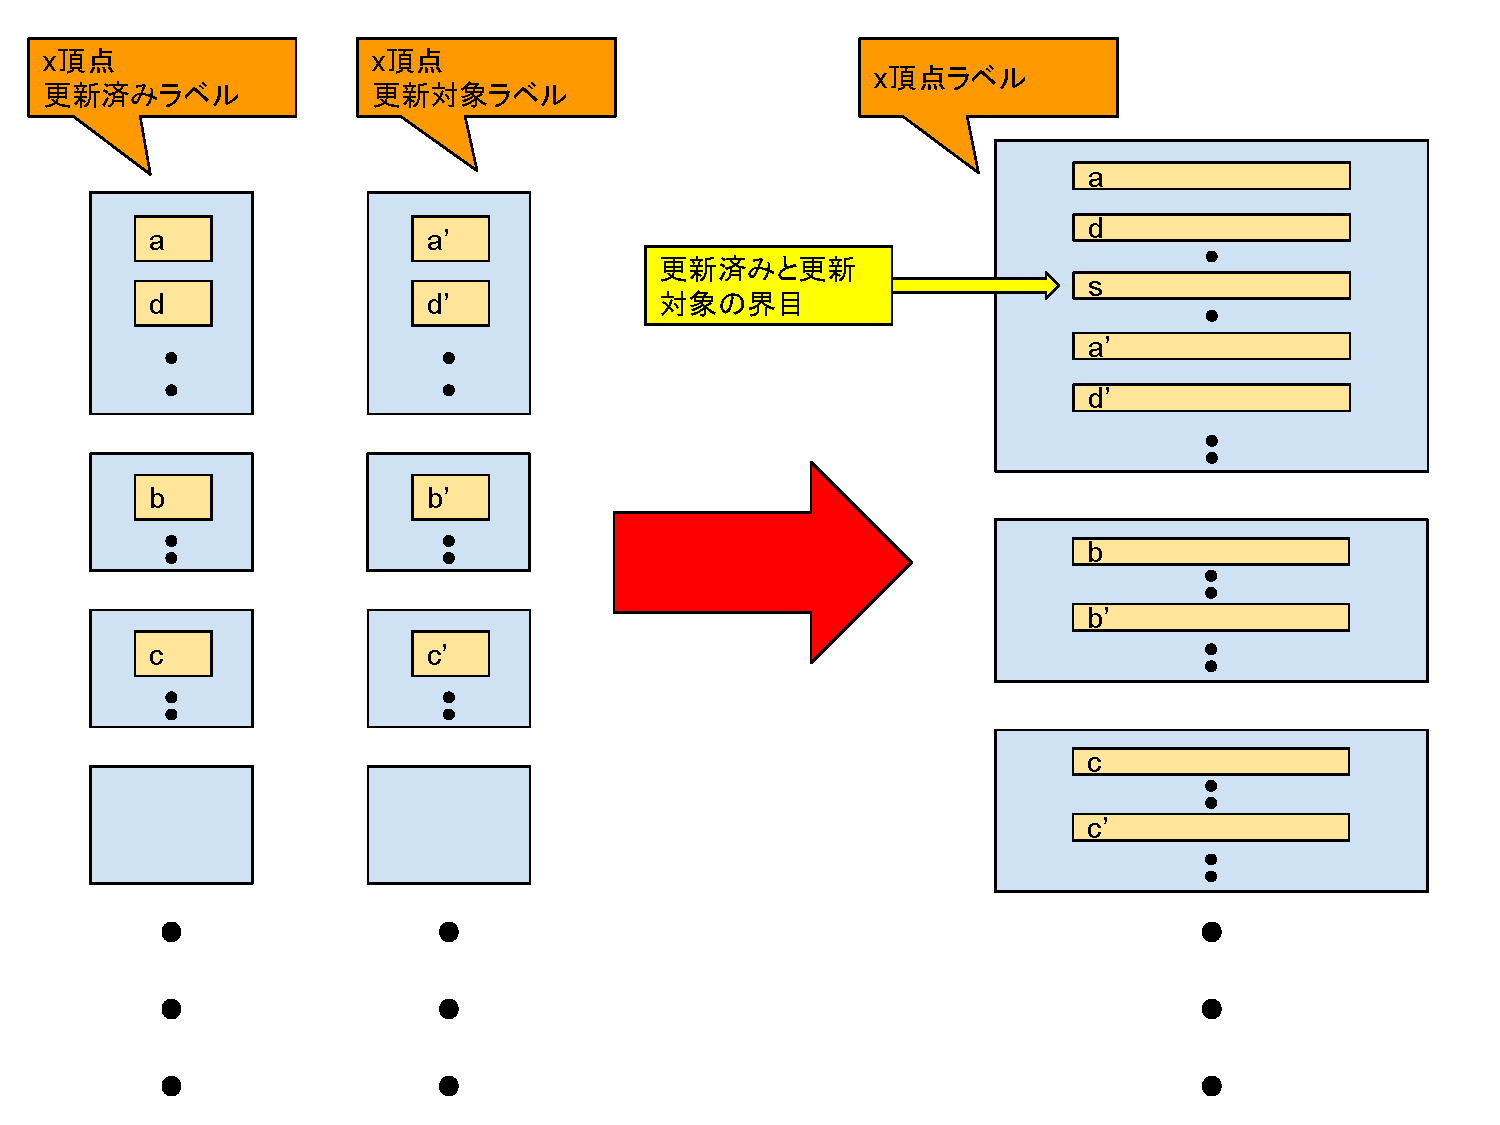
\includegraphics[width=10.0cm]{fig/fig4.pdf}
\end{figure}

完全多項式時間近似スキームによる解法とラベル付けアルゴリズムによる解法を組み合わせることにより
無駄な更新を削減と解を選択するための探索の削減を実現した.これは図に示すようにいくつかのラベル
に解を分配することにより可能にしている.しかし,ラベルを複数作ってしまうとメモリを多く使ってしまう.
この問題を解決するために任意の頂点に対する更新済みのラベルと更新対象のラベルの結合を考える.
具体的には,更新済みラベルの後ろに更新対象とするラベルを結合し,更新対象とするラベルの先頭
を記憶していく.通常,更新対象となる解は後に更新済みの解となり,新たな更新対象となる解が発見される.
つまり,更新対象となる解をラベルの後ろに加えていくことで更新済みの解の前に更新対象となる解
が来ることはない.このため,更新対象となる先頭の解を記憶しておけば,その後に続く解は全て更新対象
となる解である.図4.2に示すように解$s$を更新対象となる先頭の解とすると,その後にある解$a',d'$
は更新対象となる解である.
以下にアルゴリズムを記載する.

\begin{quote}
  \textbf{記号}
  \begin{description}
    \item[$k$:] 最適化目的の数
    \item[$v \in V$に対して]
    \item[$L_v$:] 頂点$v$に対するラベル
    \item[$M(L_v)$:] 頂点$v$に対するラベルにおいて,更新対象とその他の境界となる解
    ($M(L_v)$が$L_v$のi番目の解のとき,i+1番目以降の解は更新対象とする)
    \item[$v \in V$,$j = 1 , \ldots , k$に対して]
    \item[$l_{jv}$:] 始点からノード$v$に到達したときに生じる
    第$j$番目の目的関数における総コスト
    \item[$e \in E$,$j = 1 , \ldots , k$に対して]
    \item[$e_{jw}$:] 辺$e$の第$j$番目の目的関数におけるコスト
  \end{description}
\end{quote}

\begin{quote}
  \textbf{アルゴリズム}
  \begin{description}
    \item[入力:] グラフ$G=(V,E)$,始点$s \in V$,最適化目的の数$k$,
    各辺の重みを返す関数$w : E \to \mathbb{R}^k$
    \item[出力:] $s$から全ての頂点への最短経路となるパレート解の集合
    \item[Step 1.] $\forall v \in V , L_v \leftarrow \emptyset$,
    $L_s \leftarrow (s,0,\ldots,0)$
    \item[Step 2.] 更新ができなくなるまで以下の操作を行う.
    \begin{description}
      \item[Step 2-1.] $\forall v \in V$となる頂点$v$に対して以下の操作を行う.
      \begin{description}
        \item[Step 2-1-1.] $\forall u \in V$となる頂点$u$に対して以下の操作を行う.
        \begin{description}
          \item[Step 2-1-1-1.] $L_v$から$L_u$に対しての更新を行う.
        \end{description}
        \item[Step 2-1-2.] $M(L_v)$を$L_v$の最後の解とする.
      \end{description}
    \end{description}
    \item[Step 3.] 全てのパレート解を出力
  \end{description}
\end{quote}

\begin{quote}
  \textbf{$L_v$から$L_u$に対しての更新}
  \begin{description}
    \item[Step 1.] $L_v$,$L_u$,頂点$v$から頂点$u$への辺$e$を受け取る.
    \item[Step 2.] $M(L_v)$より後にある全ての解$(v',l_{1v'},\ldots,l_{kv'}) \in L_v$
    について以下の操作を行う.
    \begin{description}
      \item[Step 2-1.] 辺$e$の重みベクトルを
      $\vec{e} = (e_{1w},\ldots,e_{kw})$とし,
      $(u',l_{1u'},\ldots,l_{ku'}) \leftarrow
      (u',l_{1v}+e_{1w},\ldots,l_{kv}+e_{kw})$とする.
      \item[Step 2-2.] 以下の条件を満たすとき,
      $L_u \leftarrow L_u \cup \{(u',l_{1u'},\ldots,l_{ku'})\}$とする.
      \begin{itemize}
        \item 任意の$(u^*,l_{1u^*},\ldots,l_{ku^*})\in L_u$に
        $(u',l_{1u'},\ldots,l_{ku'})$が支配されない.
        \item 任意の$(u^*,l_{1u^*},\ldots,l_{ku^*}) \in L_u$と
        $(u',l_{1u'},\ldots,l_{ku'})$における全ての目的関数値が同値でない.
      \end{itemize}
      \item[Step 2-3.] 任意の$(u'',l_{1u''},\ldots,l_{ku''})\in L_u$
      に対して$(u',l_{1u'},\ldots,l_{ku'})$が
      $(u'',l_{1u''},\ldots,l_{ku''})$を支配しているとき
      $L_u \leftarrow L_u \setminus \{(u'',l_{1u''},\ldots,l_{ku''})\}$とする.
      $(u'',l_{1u''},\ldots,l_{ku''})$の前の解が$M(L_u)$の場合,
      $(u'',l_{1u''},\ldots,l_{ku''})$の次の解を$M(L_u)$の界とする.
    \end{description}
  \end{description}
\end{quote}


\subsection{提案解法2}

問題の分析で示した通り,多目的最短経路問題はインスタンスのグラフについて辺の本数が多いほど
パレート解の数は多くなり,問題は難しくなる.つまり,インスタンスのグラフが完全グラフのとき
問題は最も難しくなる.一般的に最短経路問題では,インスタンスの重みが非負数であるグラフについて,
通る頂点数が少ないpathが解になる確率が高い.また,通る頂点数が多いpathが解になる確率は低い
(一時解となっても後に他の解に支配され削除される可能性が高い).
最適化目的の数が2,重みの幅が$w$の場合の始点$s$から終点$t$への最短経路を求める.
頂点$v$を経由した$s$から$t$への経路(経由頂点数が1の経路)を$(s,v,t)$と表す.
頂点$v_1,\ldots,v_10$を経由した$s$から$t$への経路(経由頂点数が10の経路)
を$(s,v_1,\ldots,v_10,t)$と表す.$(s,v,t)$の各目的関数の値の幅は$[0,2w]$であり,
$(s,v_1,\ldots,v_10,t)$の各目的関数の値の幅は$[0,11w]$となる.
$[0,11w]$の値が$[0,2w]$の値となるとなる確率は2/11であるため$[0,2w]<[0,11w]$となる確率は高いと言える.
よって,$(s,v,t)$の各目的関数が$(s,v_1,\ldots,v_10,t)$の各目的関数より低くなる確率が高いので
$(s,v_1,\ldots,v_10,t)$が解になる確率が低く,$(s,v,t)$が解になる確率は高い.
解とならないpathを先に探索してしまうと,解となっても後に削除されるpathを更新対象としてしまい,
更新する無駄作業と削除する無駄作業が生じてしまう.
以上より,経由する頂点数が少ないpathから順に探索した方が効率的だと考えられる.


\begin{figure}[htbp]
  \centering
  \caption{提案解法1による探索}
  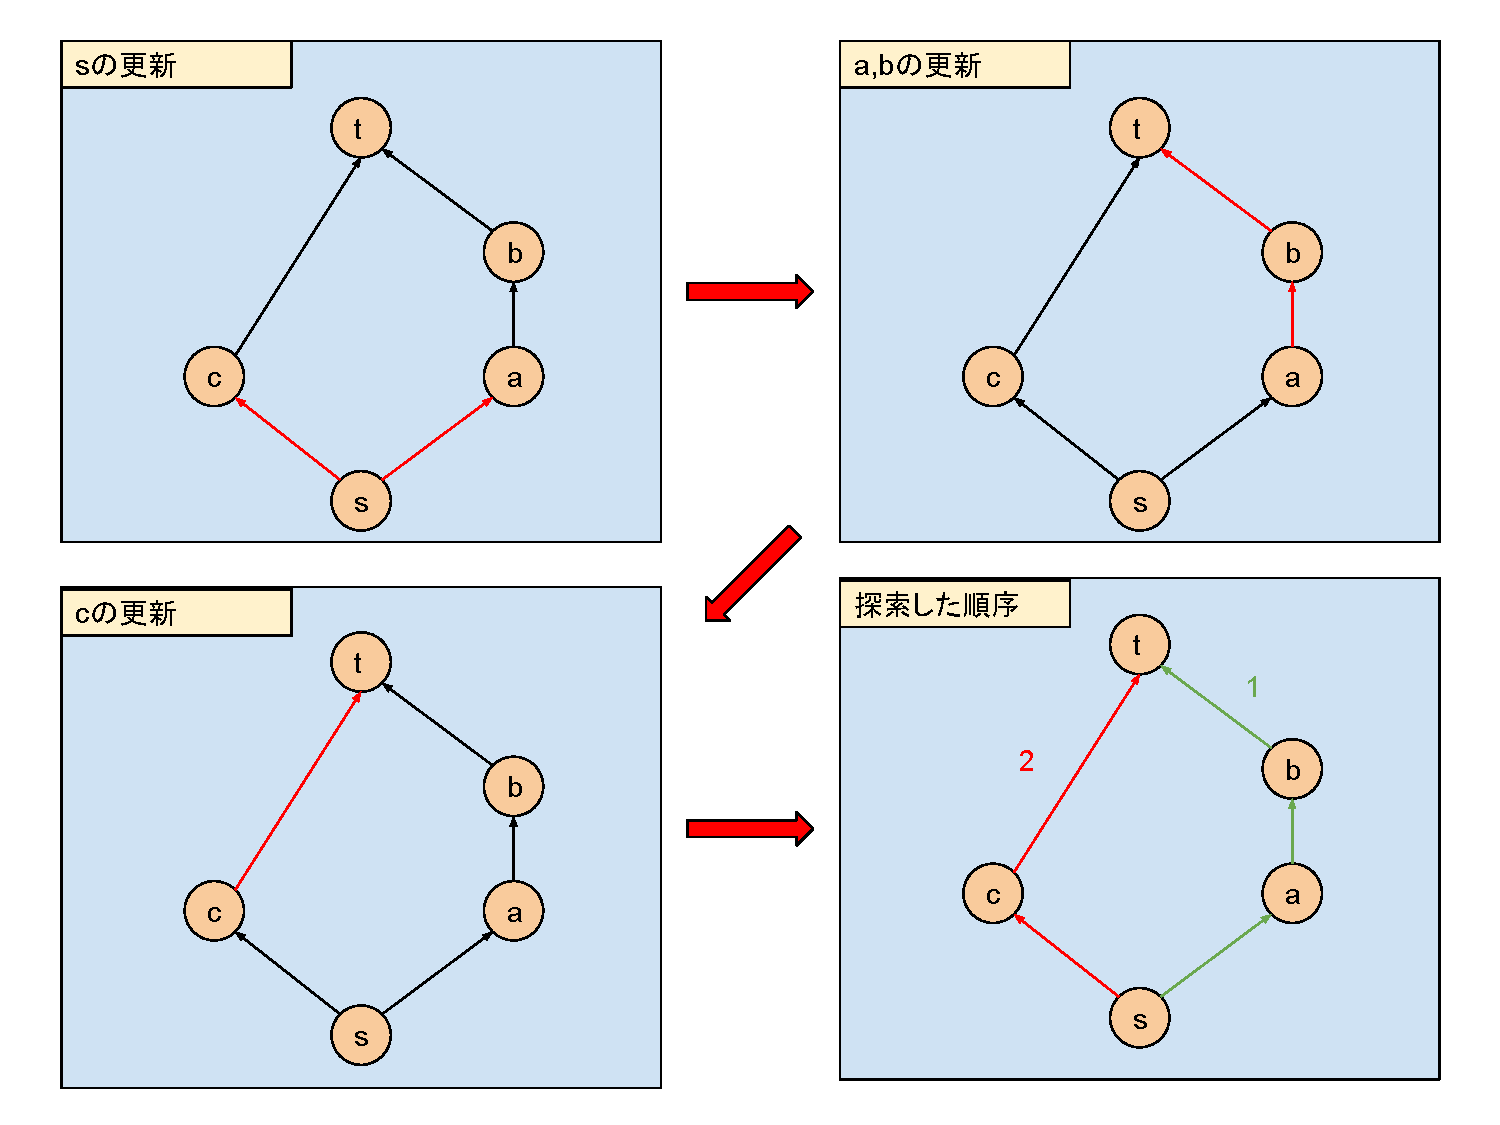
\includegraphics[height=6.0cm, width=8.0cm]{fig/fig6.pdf}
\end{figure}

図4.3に示したように提案解法1の探索順序では経由する頂点が多いpathが経由する頂点が少ないpath
よりも先に見つかってしまい1度ラベルに含まれてしまう.経由する頂点が多いpathは経由する頂点が少ないpath
よりも解になる確率は低いため,経由する頂点が少ないpathがあとで探索されたとき経由する頂点が多いpathは削除
される可能性がある.また,後に削除されるpathに対して更新して求められたpathはパレート最適解とならない.
後に削除されるpathを$a$,$a$を支配するpathを$b$,$a$の更新によって求まるpathを$a'$,$b$の更新によって求まるpathを$b'$
とする.更新に使った辺を$e$とすると,$a',b'$はそれぞれ$a,b$の各目的関数に$e$の重みベクトルの値と足したものとなる.
つまり,$a'=a+e,b'=b+e$が成り立つ.よって, $a$が$b$に支配されるとき$a'$は$b'$に支配されるため,
後に削除されるpathに対して更新して求められたpathはパレート最適解とならない.
pathに対して1度ラベルに含んだあと削除することや,後に削除されるpathに対して更新を行う
という作業は無駄なため提案解法1の探索順序は非効率であると考えられる.

\begin{figure}[htbp]
  \centering
  \caption{提案1と提案解法2のラベル比較}
  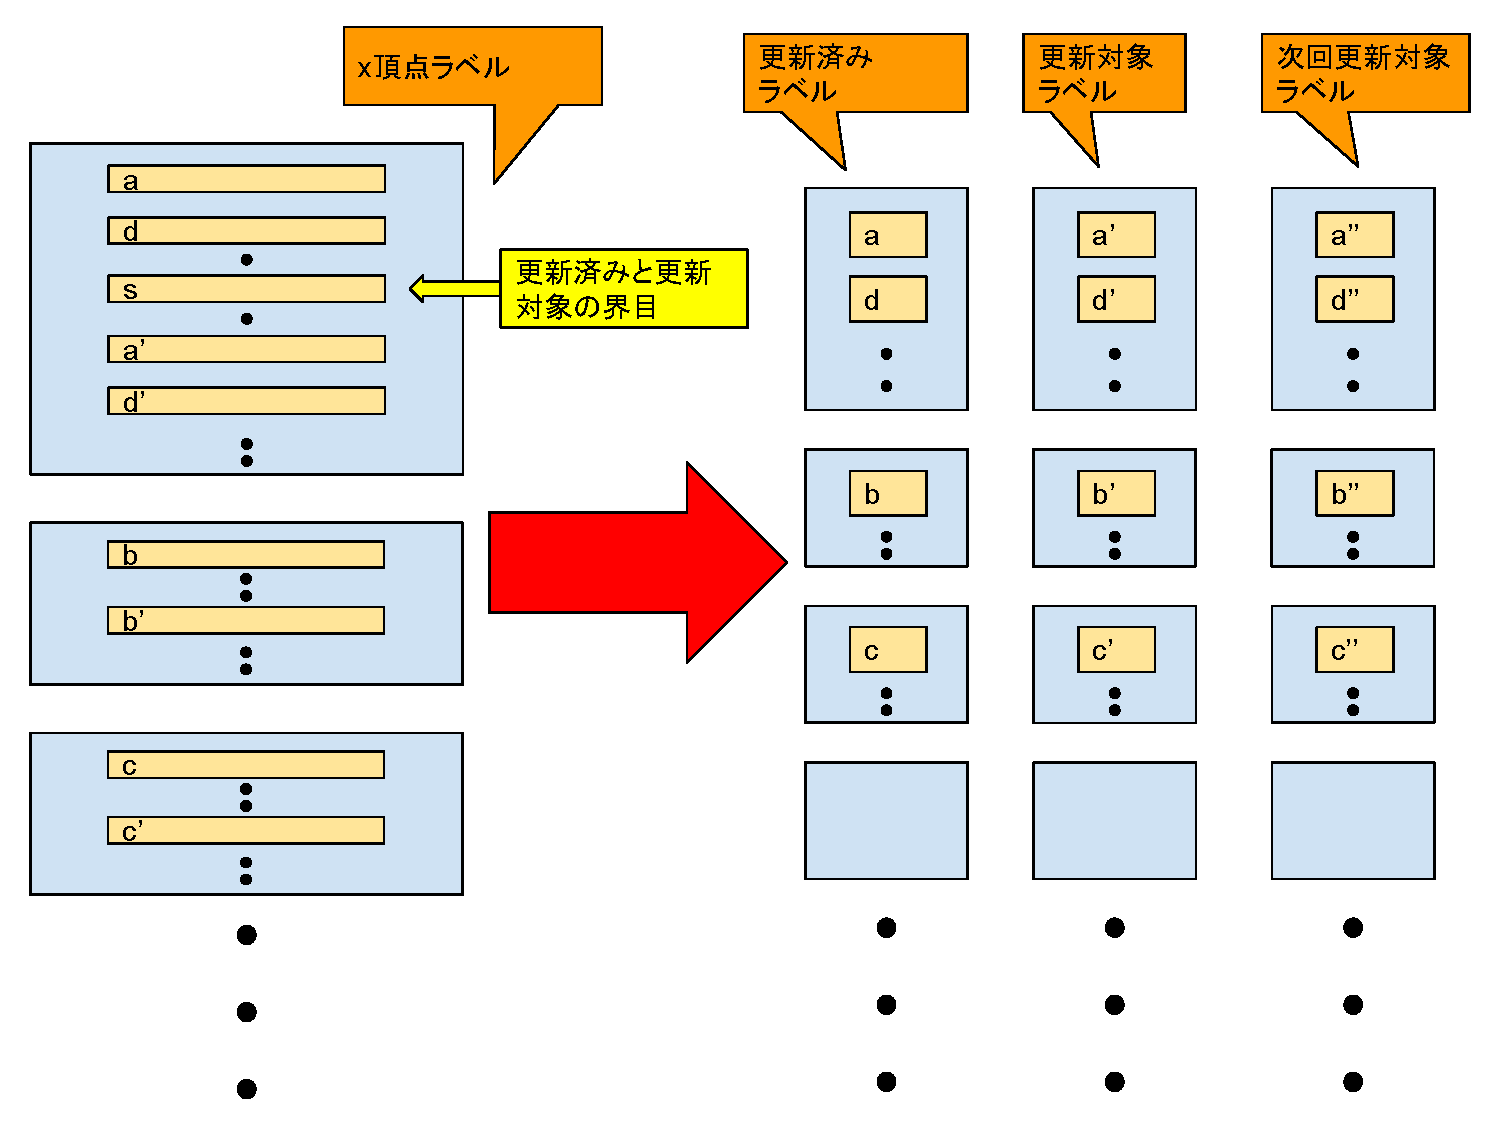
\includegraphics[width=10.0cm]{fig/fig8.pdf}
\end{figure}

非効率である提案解法1の探索順序の改善方法を考える.すでに示した通り提案解法1の探索順序では経由する
頂点が多いpathが経由する頂点が少ないpathよりも先に見つかってしまい1度ラベルに含まれてしまう.
つまり,経由する頂点が少ないpathが経由する頂点が多いpathよりも先に見つかるようにしたい.
まず,提案解法1でそのようになる原因を考える.提案解法1の探索順序では1回の更新で全ての頂点に存在する
更新対象となるpathを更新するが,更新する頂点の順序によって経由する頂点が多いpathが更新されてしまう.
例えば完全グラフにおいて頂点$a,b$を更新するとき,$a$を先に更新したとすると$b$には$a$に対するpathを
更新して得られたpathが更新対象となるpathとして保存されているため$b$の更新の際に$a$を経由して得られたpath
(経由する頂点数が多いpath)を更新してしまう.この問題を解決するために1回の更新内で得られたpath
(経由する頂点数が多いpath)を別で保存し,全頂点に対する更新が終わった時点で更新対象となるpathとする.
これにより,全体の中で最長のpath(経由する頂点数が多いpath)は今までに行なった前回に対する更新の回数となり,
経由する頂点が多いpathが経由する頂点が少ないpathよりも先に発見されることはない.

\begin{figure}[htbp]
  \centering
  \caption{提案解法2による探索}
  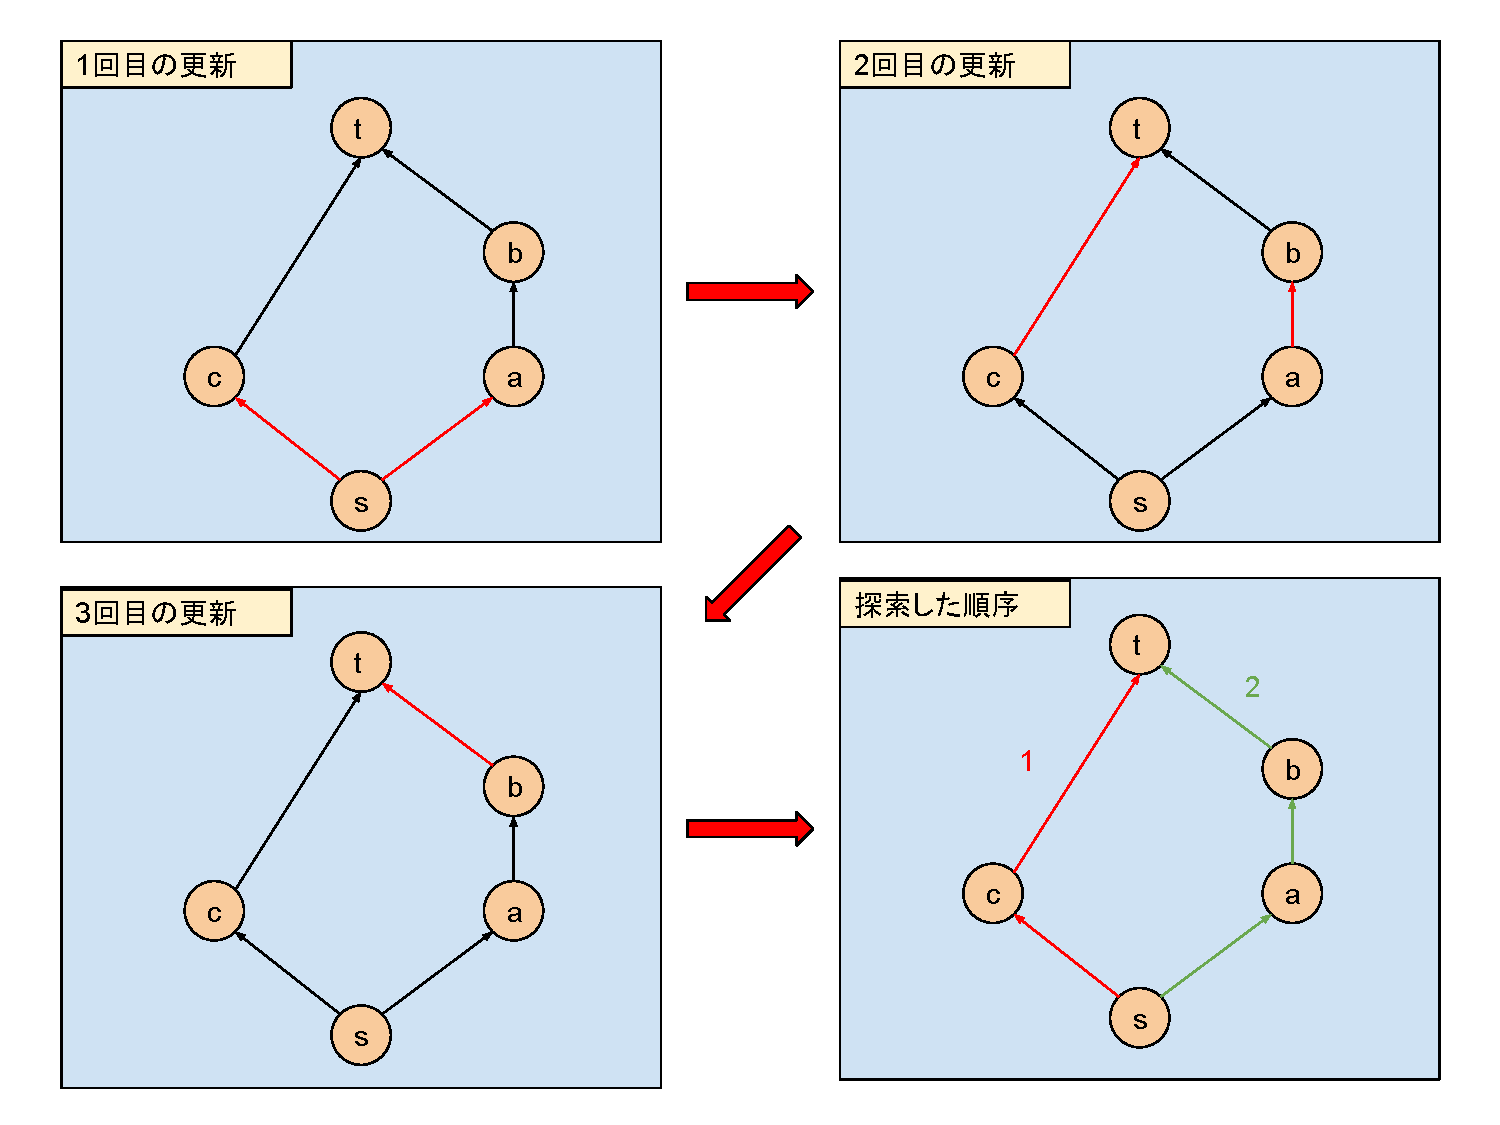
\includegraphics[height=6.0cm, width=8.0cm]{fig/fig7.pdf}
\end{figure}

この探索方法により経由する頂点が多いpathが経由する頂点が少ないpathよりも先に発見されることはなくなり,
1度解となったpathが後に削除される確率は低くなったので全体のpathに対する更新は少なくなると考えられる.
しかし,1回の更新内で得られたpath(経由する頂点数が多いpath)を別で保存し,全頂点に対する更新が終わった時点で
更新対象となるpathとすることにより1回の更新に要する実装時間は長くなる.提案解法1では更新対象となるpathを
更新対象としないpathに移動させるだけだったが,提案解法2ではそれらに加えて更新内で得られたpathを更新対象とするapth
に移動させるという作業が増える.そのため,提案解法2が提案解法1に比べて一定以上全体のpathに対する更新は少なくなら
なければ非効率となってしまう.つまり,提案解法2が提案解法1に比べて一定以上削除される解を減らさなければならない.
以下にアルゴリズムを記載する.

\begin{quote}
  \textbf{記号}
  \begin{description}
    \item[$k$:] 最適化目的の数
    \item[$v \in V$に対して]
    \item[$L_{vx}$:] 頂点$v$に対する,更新対象としないラベル
    \item[$L_{vy}$:] 頂点$v$に対する,更新対象とするラベル
    \item[$L_{vz}$:] 頂点$v$に対する,次回探索で更新対象とするラベル
    \item[$v \in V$,$j = 1 , \ldots , k$に対して]
    \item[$l_{jv}$:] 始点からノード$v$に到達したときに生じる
    第$j$番目の目的関数における総コスト
    \item[$e \in E$,$j = 1 , \ldots , k$に対して]
    \item[$e_{jw}$:] 辺$e$の第$j$番目の目的関数におけるコスト
  \end{description}
\end{quote}

\begin{quote}
  \textbf{アルゴリズム}
  \begin{description}
    \item[入力:] グラフ$G=(V,E)$,始点$s \in V$,最適化目的の数$k$,
    各辺の重みを返す関数$w : E \to \mathbb{R}^k$
    \item[出力:] $s$から全ての頂点への最短経路となるパレート解の集合
    \item[Step 1.] $\forall v \in V , L_v \leftarrow \emptyset$,
    $L_{sy} \leftarrow (s,0,\ldots,0)$
    \item[Step 2.] 更新ができなくなるまで以下の操作を行う.
    \begin{description}
      \item[Step 2-1.] $\forall v \in V$となる頂点$v$に対して以下の操作を行う.
      \begin{description}
        \item[Step 2-1-1.] $\forall u \in V$となる頂点$u$に対して以下の操作を行う.
        \begin{description}
          \item[Step 2-1-1-1.] $L_{vy}$から$L_u$に対しての更新を行う.
        \end{description}
      \end{description}
      \item[Step 2-2.] $\forall v \in V$に対して
      $L_{vx},L_{vy},L_{vz}$の更新を行う.
    \end{description}
    \item[Step 3.] 全てのパレート解を出力
  \end{description}
\end{quote}

\begin{quote}
  \textbf{$L_{vy}$から$L_u$に対しての更新}
  \begin{description}
    \item[Step 1.] $L_{vy}$,$L_u$,頂点$v$から頂点$u$への辺$e$を受け取る.
    \item[Step 2.] $\forall (v',l_{1v'},\ldots,l_{kv'}) ,
    (v',l_{1v'},\ldots,l_{kv'}) \in L_{vy}$について以下の操作を行う.
    \begin{description}
      \item[Step 2-1.] 辺$e$の重みベクトルを
      $\vec{e} = (e_{1w},\ldots,e_{kw})$とし,
      $(u',l_{1u'},\ldots,l_{ku'}) \leftarrow
      (u',l_{1v}+e_{1w},\ldots,l_{kv}+e_{kw})$とする.
      \item[Step 2-2.] 以下の条件を満たすとき,
      $L_{uz} \leftarrow L_{uz} \cup \{(u',l_{1u'},\ldots,l_{ku'})\}$とする.
      \begin{itemize}
        \item 任意の$(u^*,l_{1u^*},\ldots,l_{ku^*})\in \{L_{ux} \cup L_{uy} \cup L_{uz}\}$に
        $(u',l_{1u'},\ldots,l_{ku'})$が支配されない.
        \item 任意の$(u^*,l_{1u^*},\ldots,l_{ku^*}) \in \{L_{ux} \cup L_{uy} \cup L_{uz}\}$と
        $(u',l_{1u'},\ldots,l_{ku'})$における全ての目的関数値が同値でない.
      \end{itemize}
      \item[Step 2-3.] 任意の$(u'',l_{1u''},\ldots,l_{ku''})\in L_{ux}$
      に対して$(u',l_{1u'},\ldots,l_{ku'})$が
      $(u'',l_{1u''},\ldots,l_{ku''})$を支配しているとき
      $L_{ux} \leftarrow L_{ux} \setminus \{(u'',l_{1u''},\ldots,l_{ku''})\}$とする.
      \item[Step 2-4.] 任意の$(u'',l_{1u''},\ldots,l_{ku''})\in L_{uy}$
      に対して$(u',l_{1u'},\ldots,l_{ku'})$が
      $(u'',l_{1u''},\ldots,l_{ku''})$を支配しているとき
      $L_{uy} \leftarrow L_{uy} \setminus \{(u'',l_{1u''},\ldots,l_{ku''})\}$とする.
      \item[Step 2-5.] 任意の$(u'',l_{1u''},\ldots,l_{ku''})\in L_{uz}$
      に対して$(u',l_{1u'},\ldots,l_{ku'})$が
      $(u'',l_{1u''},\ldots,l_{ku''})$を支配しているとき
      $L_{uz} \leftarrow L_{uz} \setminus \{(u'',l_{1u''},\ldots,l_{ku''})\}$とする.
    \end{description}
  \end{description}
\end{quote}

\begin{quote}
  \textbf{$L_{vx},L_{vy},L_{vz}$の更新}
  \begin{description}
    \item[Step 1.] $L_{vx},L_{vy},L_{vz}$を受け取る.
    \item[Step 2.] $L_{vx} = L_{vx} \cup L_{vy}$とし,
    $L_{vy} = \{ \emptyset \}$とする.
    \item[Step 3.] $L_{vy} \leftarrow L_{vz}$とし,
    $L_{vz} = \{ \emptyset \}$とする.
  \end{description}
\end{quote}


\section{負の値の考慮した問題に対する解法の提案}

単目的最短経路問題では負の閉路が存在する場合,負の閉路の存在を報告し最短経路は求めなかった.
これは負の閉路を何度も通過することによって重みを更新し続けるためである.しかし,多目的最短経路問題の場合,
目的関数が複数存在するので1つの目的関数において負の閉路が存在する場合でも,他の目的関数による最適化をすることで
解を求めることができる.よって,本研究では負の閉路が存在する目的関数を考慮しない解を求める.
単目的最短経路問題におけるベルマンフォード法では,$|V|$回目の更新を行うことによって負の閉路が存在するか
の判定をし報告を行なっていた.しかし,本研究では負の閉路が存在するとき負の閉路が存在しない目的関数に対しての
解を求めるため,どの目的関数において負の閉路が存在しているのかを確かめる必要がある.また,負の閉路が存在するとき
単目的最短経路問題よりも多くの実装時間を要してしまう.単目的最短経路問題では全体の解の数が最大で頂点数$|V|$のため
1回の探索で最大で$|V|$つのpathの更新で済むが,多目的最短経路問題では全体の解の数が最大で
$\displaystyle \sum_{i=0}^{n-1} {}_{(n-1)}C_i i!$つ存在するため1回の探索で更新するpathは多くなるため
$|V|$回目の更新を行うまでに多くの実装時間がかかってしまう.これらの問題を解決するために負の値の考慮した問題に対する
解法の提案を行う.また,提案解法2に基づいた解法を提案する.
ある目的関数において負の閉路が存在する場合,その目的関数を削除する.目的関数の削除は以下の手順で行こなわれる.

\begin{description}
  \item[探索途中で負の閉路を検出]
\end{description}

単目的最短経路問題では全体の解の数が最大で頂点数$|V|$のため1回の探索で最大で$|V|$つのpathの更新で済むが,
多目的最短経路問題では全体の解の数が最大で$\displaystyle \sum_{i=0}^{n-1} {}_{(n-1)}C_i i!$つ存在するため
1回の探索で更新するpathは多くなるため$|V|$回目の更新を行うまでに多くの実装時間がかかってしまうという問題に対して,
探索途中で負の閉路を検出する方法を提案する.探索途中で負の閉路を検出することにより$|V|$回目の更新を行う必要がなくなり,
$|V|$回目の更新を行うまでにかかる多くの実装時間が削減される.探索途中で負の閉路を検出する方法としては,提案解法2における
Step 2-1-1-1で負の閉路が存在するかの判定をし,1回の全体に対する更新が終わった時点で負の閉路が存在する場合,その目的関数を削除する.
負の閉路が存在するかの判定は解となったpathが閉路となっているかで判定する.pathが閉路となっている場合,同じ頂点を2回通っている
ということである.同じ頂点を2回通っているpathが解となるとき,その頂点を1回通ったpathに2回通ったpathが支配されていない状態
なので,任意の目的関数において2回通ったpathの値が1回通ったpathの値よりも低くなっている.2回通ったpathの値が1回通ったpathの値
よりも低くなっているということは3回通ったparhも2回通ったpathよりも低い値となり,負の閉路となる.よって,解となったpathが閉路となっているかで
負の閉路の存在を判定できる.また,どの目的関数が低くなっているかを求めることで負の閉路の原因となっている目的関数を特定できる.

\begin{quote}
  \textbf{目的関数$k_1$の削除}
  \begin{description}
    \item[Step 1.] $k_1,E,L$(全てのラベル)を受け取る.
    \item[Step 2.] $\forall e \in E$について$\vec{e}={f_1,\ldots,f_k}$とし,$k_1$に対応する値が
    $f_1$のとき,$f_1=0$とする.
    \item[Step 3.] $\forall l \in L$について$\vec{l}={f_1,\ldots,f_k}$とし,$k_1$に対応する値が
    $f_1$のとき,$f_1=0$とする.
    \item[Step 4.] $\forall l \in L$について$l$が解であるかの判定をする.
  \end{description}
\end{quote}

\begin{quote}
  \textbf{$l$が解であるかの判定}

  以下の条件を満たすとき$L=L \setminus \{ l\}$
    \begin{itemize}
      \item 任意の$l' \in L$に$l$が支配される.
      \item 任意の$l' \in L$と$l$における全ての目的関数値が同値である.
    \end{itemize}
\end{quote}

\begin{description}
  \item[負の閉路探索を行なった後探索をする]
\end{description}

どの目的関数において負の閉路が存在しているのかを確かめる必要があり,単目的最短経路問題では全体の解の数
が最大で頂点数$|V|$のため1回の探索で最大で$|V|$つのpathの更新で済むが,多目的最短経路問題では全体の解の数が最大で
$\displaystyle \sum_{i=0}^{n-1} {}_{(n-1)}C_i i!$つ存在するため1回の探索で更新するpathは多くなるため
$|V|$回目の更新を行うまでに多くの実装時間がかかってしまうという2つの問題を解決するために負の閉路探索を行なった後探索をする
方法を提案する.探索前に負の閉路を検出することにより$|V|$回目の更新を行う必要がなくなり,
$|V|$回目の更新を行うまでにかかる多くの実装時間が削減される.探索前に負の閉路を検出する方法としては,提案解法2における
Step 1の前で負の閉路が存在するかの判定をし,負の閉路が存在する場合その目的関数を削除する.負の閉路が存在するかの判定
は各目的関数に対して単目的最短経路問題のベルマンフォード法を実行する.単目的最短経路問題のベルマンフォード法は
$|V|$回の更新を行うが,1回の更新で最大でも$|V|$つの更新しか行わないため短い時間で負の閉路の探索ができる.
また,各目的関数ごとに負の閉路判定ができるため,どの目的関数において負の閉路が存在するのか分かる.


\begin{quote}
  \textbf{目的関数$k_1$の削除}
  \begin{description}
    \item[Step 1.] $k_1,E,L$(全てのラベル)を受け取る.
    \item[Step 2.] $\forall e \in E$について$\vec{e}={f_1,\ldots,f_k}$とし,$k_1$に対応する値が
    $f_1$のとき,$f_1=0$とする.
  \end{description}
\end{quote}

\begin{description}
  \item[負の閉路探索結果で求めた解を利用して探索をする]
\end{description}

前に提案した負の閉路探索を行なった後探索をする方法を改良する.負の閉路探索を行なった後探索をする方法では
探索した解は保存せずに最初から探索を行なっていた.しかし,負の閉路で探索した解は少しの工夫で必ずパレート
最適解に含まれるため,負の閉路探索結果で求めた解を利用して探索をする方法を提案する.
最終的にパレート最適解でない解を利用して探索してしまうと,求めた解を利用して探索して得られた解が削除
されてしまうため無駄な探索となってしまう.よって,負の閉路探索結果で求めた解を利用して探索をする場合
確実にパレート最適解となる解を求めて探索をしなければならない.
各目的関数に対して負の閉路探索で得た解はその目的関数の値に対して低くなるpathは存在しない.しかし,
その目的関数の値が同じで他の目的関数が得た解より低い場合,得た解は支配されてしまいパレート最適解ではなくなってしまう.
そのため,同じ値であるpathが得られた場合は他の目的関数の比較をし,優位な方を選択する必要がある.
これにより,得られた解は必ずパレート解になるため求めた解を利用して探索をすることが可能になる.
この解法は提案解法2に以下を付け加える.

\begin{quote}
  \begin{description}
    \item[Step 0.] 各目的関数に対して以下の操作を行う.
    \begin{description}
      \item[Step 0-1.] $s_w = 0$とし,$v \in V/\{s\}$に対して$v_w = \infty$とする.
      \item[Step 0-2.] $|V|-1$ 回以下の操作を行う.
      \begin{description}
        \item[Step 0-2-1.] $e = {e \in E \mid v,u \in e}$となる$e$に対して,
        $u_w > v_w + e_w$を満たすとき以下の操作を行う.
        \begin{description}
          \item[Step 0-2-1-1.] $u_w = v_w + e_w$.
        \end{description}
        \item[Step 0-2-2.] $e = {e \in E \mid v,u \in e}$となる$e$に対して,
        $u_w = v_w + e_w$を満たすとき以下の操作を行う.
        \begin{description}
          \item[Step 0-2-2-1.] $u_w$となるpathが$v_w + e_w$となるpathに支配されるとき,
          $u_w = v_w + e_w$.
        \end{description}
      \end{description}
      \item[Step 0-3.] Step 0-2-1を行いノードの重みが更新された場合,その目的関数を削除する.
    \end{description}
  \end{description}
\end{quote}

\begin{quote}
  \textbf{目的関数$k_1$の削除}
  \begin{description}
    \item[Step 1.] $k_1,E,L$(全てのラベル)を受け取る.
    \item[Step 2.] $\forall e \in E$について$\vec{e}={f_1,\ldots,f_k}$とし,$k_1$に対応する値が
    $f_1$のとき,$f_1=0$とする.
    \item[Step 3.] $\forall l \in L$について$\vec{l}={f_1,\ldots,f_k}$とし,$k_1$に対応する値が
    $f_1$のとき,$f_1=0$とする.
    \item[Step 4.] $\forall l \in L$について$l$が解であるかの判定をする.
  \end{description}
\end{quote}

\section{実装における工夫}

\begin{description}
  \item[リストの工夫]
\end{description}

単目的最短経路問題では各頂点が1つの解(path)しか持たないが,多目的最短経路問題では各頂点がパレート最適解として複数の解を
持つ.そこで,複数の解を保存しておくリストを作成する.リストは解の集合である.多目的最短経路問題では1度解となったpathが
後に発見されるpahtによって支配され削除されることがある.よって,リストを作成する際,効率的に解を削除することを考慮する.
また,提案解法1では順序つきの集合として定義する必要がある.順序つきの集合として定義することによって更新する解をリストの前から
選択していくことでどの解を選択していくかという作業がなくなるため提案解法2でも有効的に使用できる.

\begin{description}
  \item[ArrayList]
\end{description}

ArrayListは配列を利用したリスト構造である.ArrayListは通常の配列と異なりサイズを後からでも変更できる.
インデックス値による値の読み書きは高速である.しかし,要素の挿入/削除は,配列サイズが大きくなるほど,
また、操作位置が先頭に近くなるほど遅くなる.

\begin{figure}[htbp]
  \centering
  \caption{ArrayListのイメージ}
  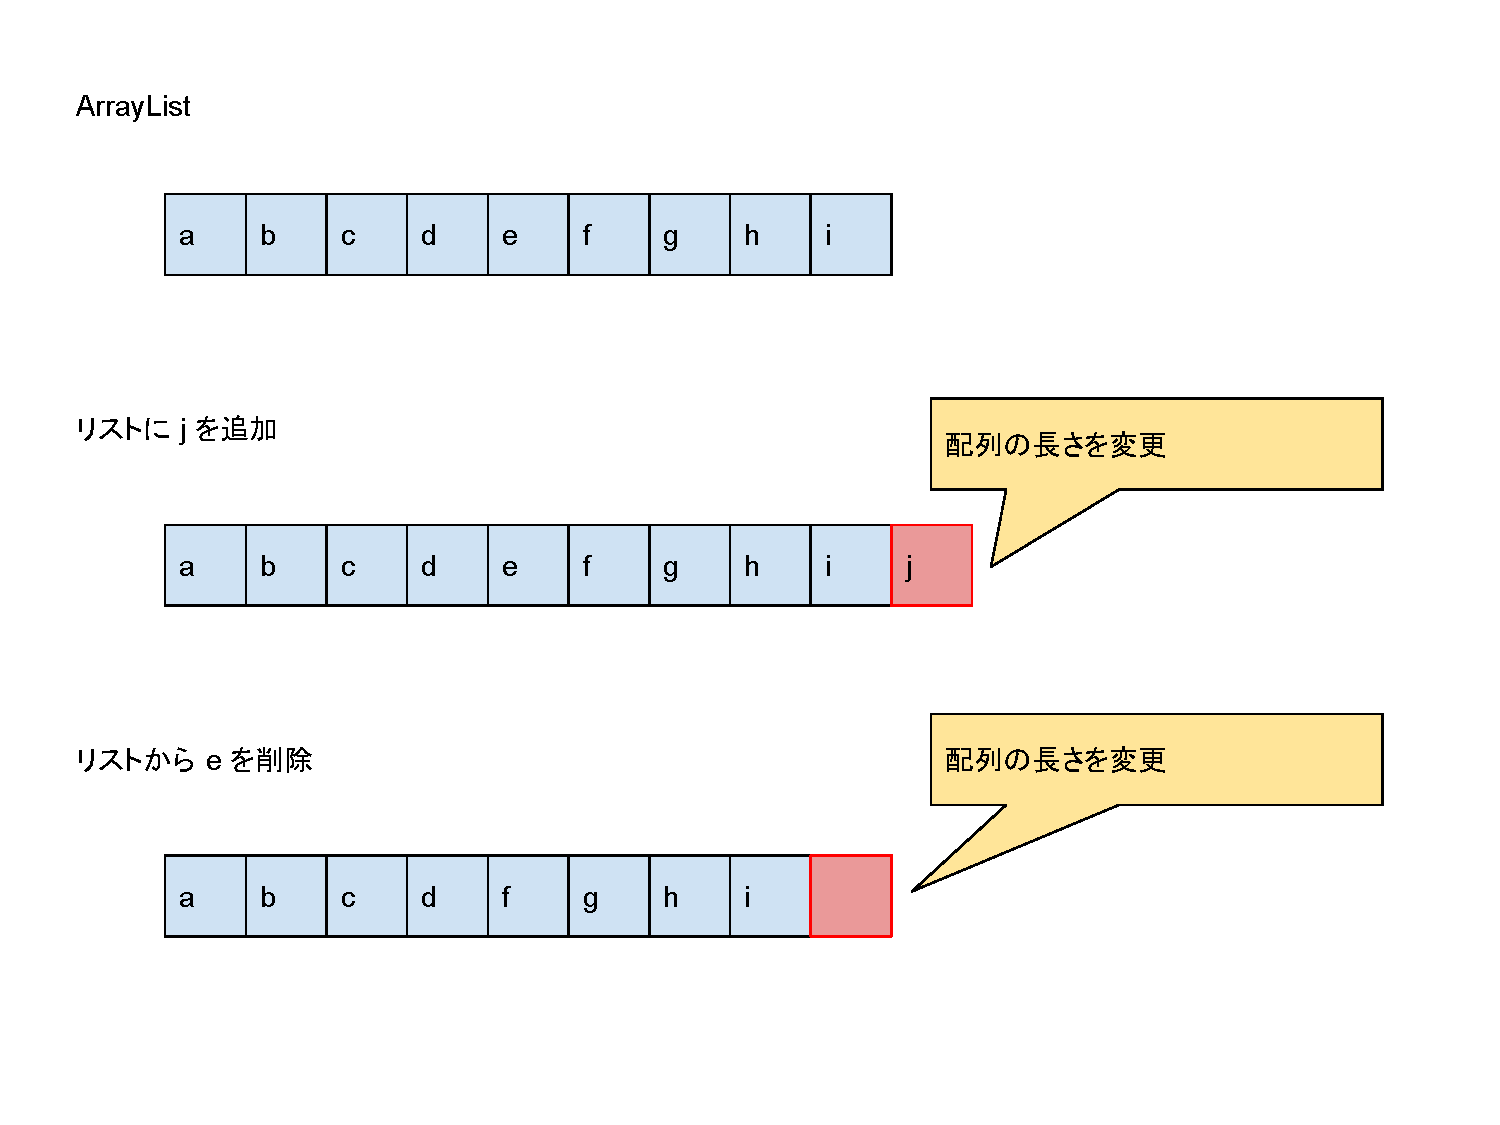
\includegraphics[height=6.0cm, width=8.0cm]{fig/fig9.pdf}
\end{figure}

提案解法1に対して,1つの頂点に対して1つのArrayListを使用する.
1つのArrayListは1つの頂点に対する解を保存しておき,更新対象としない解と更新対象とする解の界を記憶しておくことで
更新対象のする解の区別ができる.提案解法2に対して,1つの頂点に3つのArrayListを使用する.
1つの頂点に対する各ArrayListは更新対象としないもの,更新対象とするもの,次回の更新で更新ん対象にするものとする.
提案解法1では更新対象としない解と更新対象とする解の界を移動させるだけで更新対象とするものから更新対象としないものへの
解の移動が可能であるが,提案解法1では更新対象とする解を1つずつ更新対象としない解に移動させるため時間がかかる.
また,次回更新対象とする解を更新対象とする解に移動させるにも時間がかかる.解の追加/削除については配列の長さを
変更させて行うため多少の時間がかかり,削除においては削除された解の分を詰めた配列にするためさらに時間がかかる.
解の数が変わるたびに配列の長さを変えられるため事前に解の数を予測する必要がない.

\begin{description}
  \item[classを用いた双方向循環リスト]
\end{description}

双方向リストは連結リストである.各ノードは前のノードを示す後方リンクと後ろのノードを示す前方リンクを持つ.
リストの先頭のノードには前のノードがないため,後方リンクにはヌル値を格納するか空のリストを指す.
リストの最後尾のノードには次のノードがないため,前方リンクにはヌル値を格納するか空のリストを指す.
循環リストは先頭と最後尾のノードを相互に連結した連結リストである.双方向循環リストは双方向リストと循環リスト
を組み合わせたものであり,全てのノードが前のノードを示す後方リンクと後ろのノードを示す前方リンクを持つ.
双方向循環リストを用いることにより,解の追加/削除にかかる作業と解の移動にかかる作業が容易になる.

\begin{figure}[htbp]
  \centering
  \caption{双方向循環リストにおける追加/削除のイメージ}
  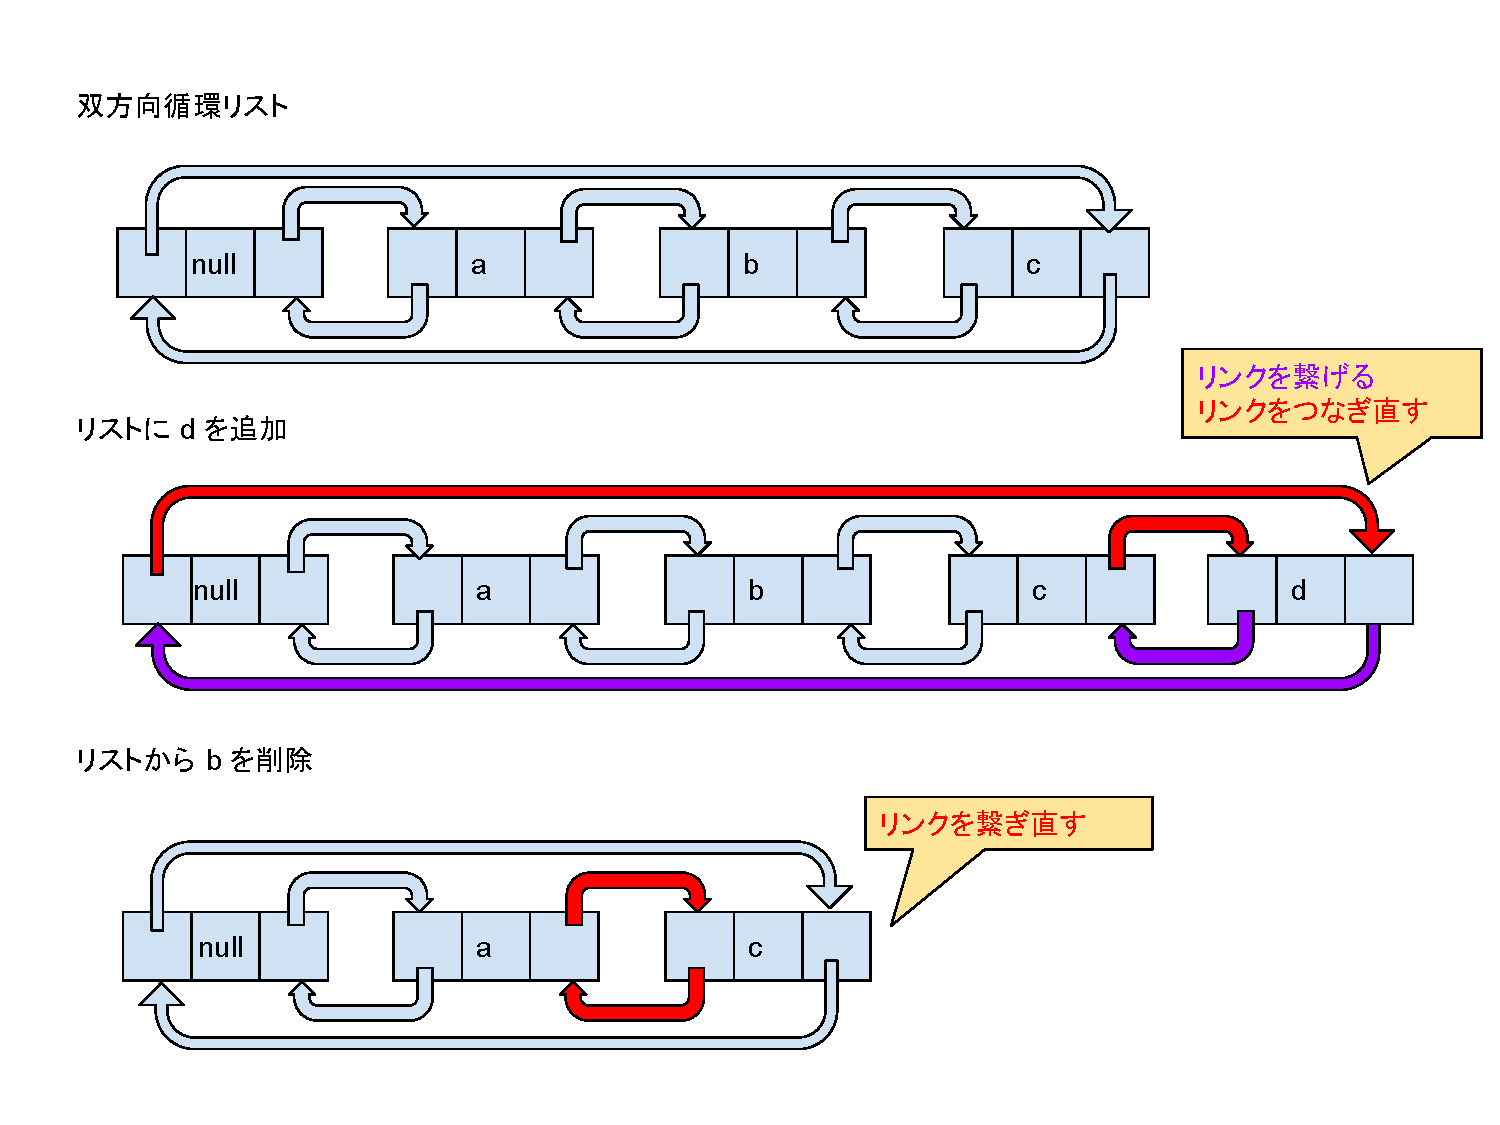
\includegraphics[height=9.0cm, width=10.0cm]{fig/fig10.pdf}
\end{figure}

双方向循環リストを用いることにより,解の追加/削除にかかる作業が容易になる理由を説明する.
リストの先頭となる空のノード(先頭の前のノードかつ最後尾のノードの後ろのノード)を$s$とする.
双方向循環リストで解をリストの最後尾に追加するとき,リストの最後尾のノードを求めるのではなく,
$s$の前のノードとして追加することができる.$s$は最後尾のノードの後ろのノードのため,$s$の前のノード
はリストの最後尾のノードとなる.よって,$s$の前のノードとして追加することで,リストの最後尾のノードの後ろ
に追加することとなる.双方向循環リストでは,リストから解を削除するとき配列のように長さを変更したり
ノードをつめるという作業が必要なくなる.リストから解を削除するときの作業は削除するノードの前のノードの
前方リンクを削除するノードの後ろのノードとし,削除するノードの後ろのノードの後方リンクを削除するノードの前のノードとする.
この操作により,リンク内に含まれる他のノードを移動させたり,リンク自体に変更を加えることがない.
以上より,双方向循環リストを用いることにより,解の追加/削除にかかる作業が容易になる.

\begin{figure}[htbp]
  \centering
  \caption{双方向循環リストにおけるリスト間の追加イメージ}
  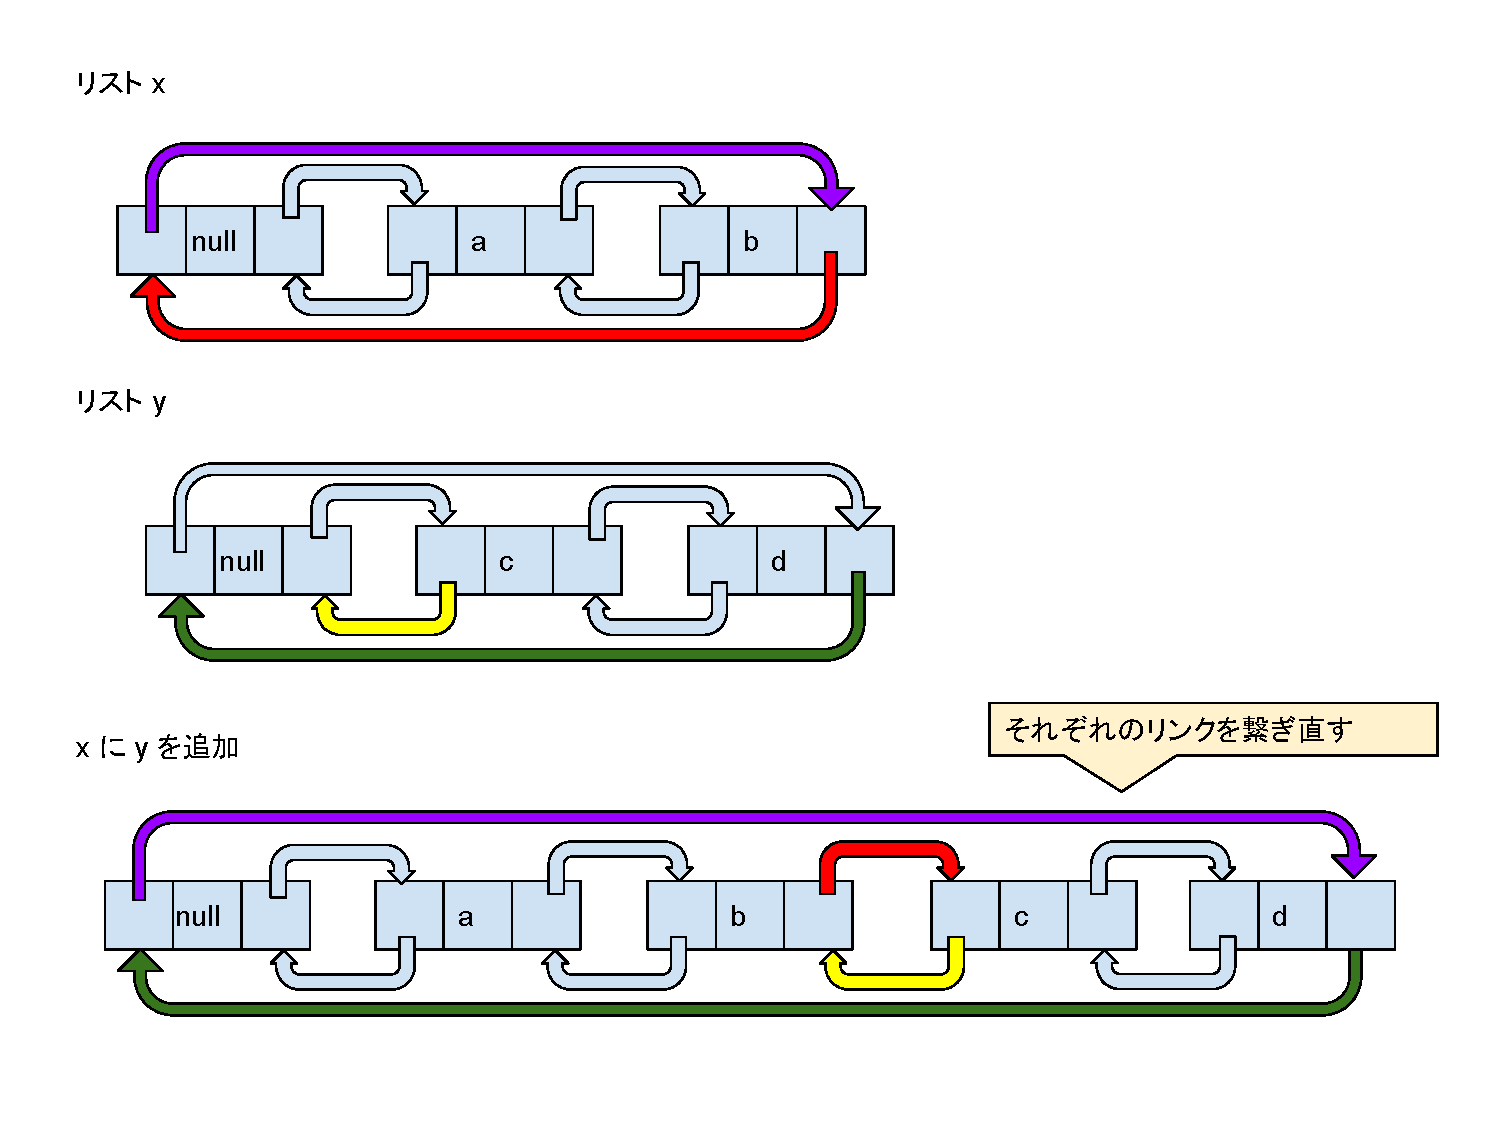
\includegraphics[height=9.0cm, width=10.0cm]{fig/fig12.pdf}
\end{figure}

双方向循環リストを用いることにより,解の移動にかかる作業が容易になる理由を説明する.
リスト$a$の要素をリスト$b$に追加することを考える.$a$の先頭となる空のノード
(先頭の前のノードかつ最後尾のノードの後ろのノード)を$a_s$とし,$b$の先頭となる空のノードを$b_s$とする.
双方向循環リストにおいて,$a$に存在するノード全てを$b$のリストの最後尾に追加するとき以下の作業を行う.
\begin{itemize}
  \item $a_s$の後ろノードの後方リンクを$b_s$の前のノードとし,$b_s$の前のノードの後方リンクを$a_s$の前のノードとする.
  \item $a_s$の前のノードの前方リンクを$b_s$とし,$b_s$の後方リンクを$a_s$の前のノードとする.
\end{itemize}
双方向循環リストでは,ノードを1つずつ移動させるのではなく4つのリンクを変更することによって全てのノードを移動させることができる.
この操作により,リンク内に含まれる他のノードを移動させたり,リンク自体に変更を加えることがない.
classを用いた双方向循環リストの場合,解(path)が発見されるたびに新しいノードを作成するため事前に解の数を予測する必要がない.


\begin{description}
  \item[配列を用いた双方向循環リスト]
\end{description}

配列を用いた双方向循環リストではclassを用いた双方向循環リスト同様双方向循環リストを使用する.
配列を用いた双方向循環リストはclassが使えないプログラミング言語(C言語等)でも使用できる.
配列を用いているため,事前に解の数を予測する必要がある.解の数が用意した配列を超える場合,
配列の長さが長い配列を作成し要素となっている解を全て移動させる必要があるため非効率となる.
配列で解を削除するときリンクを書き換えることにより可能になるが,削除される解は配列内に残ってしまう.
削除される解が配列内に残っているとメモリを大量に使用してしまうため,できるだけ削除される解が
残されない効率的な配列としたい.そのため,削除された解が存在している配列の場所を記憶しておき
解が発見されたときにその場所に格納する.解が発見されたときに毎回削除された解の場所を探し格納するのは
非効率なため,配列が全て埋まった時点で削除された解の場所を探し格納する操作を始める.この条件により,
削除された解の場所を探す回数は削減され,用意された配列を無駄にすることがない.

\begin{figure}[htbp]
  \centering
  \caption{配列を用いた双方向循環リストのイメージ}
  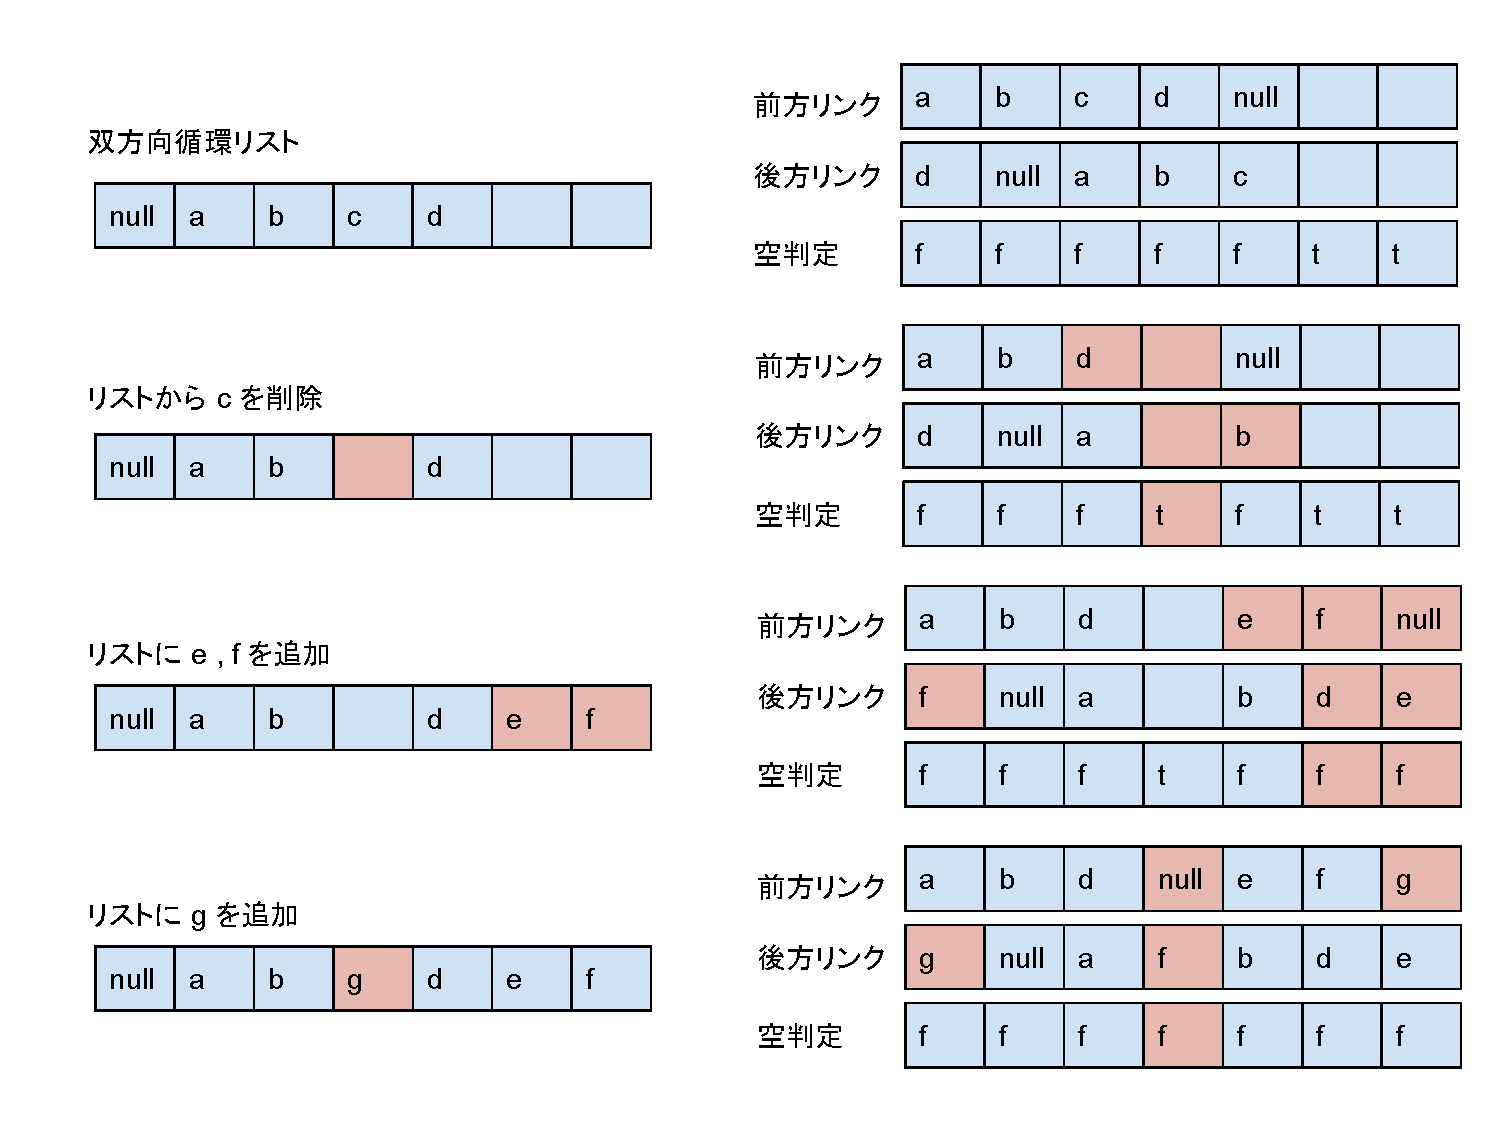
\includegraphics[height=8.0cm, width=10.0cm]{fig/fig11.pdf}
\end{figure}

\begin{description}
  \item[更新対象の工夫]
\end{description}

提案解法2では1回の更新で各頂点に対するpathを更新対象とするため,頂点を基準に更新することになる.
頂点を基準に更新するとき,その頂点から出ていく辺に対しての更新(辺の始点を更新対象とする更新)と
その頂点に入ってくる辺に対しての更新(辺の終点を更新対象とする更新)がある.それぞれの方法は
参照順序が異なるため計算時間が変わってくる.コンピュータには最後に参照したものをキャッシュに溜め込み,
次の参照が行われるときにキャッシュから取り出すことで参照時間が短くなることがある.参照時間が短く済むと
同じ比較でも実装時間が短くなるため,参照順序によっておこるキャッシュの利用が多く行われ参照時間を短くした方が良い.
そこで,それぞれの方法を実装し,計算時間の比較を行い考察を行う.

\begin{description}
  \item[辺の始点を更新対象とする]
\end{description}

辺の始点を更新対象とする場合を考える.辺の始点を更新対象としたとき更新対象となる頂点から出ていく辺
に対して拡張探索を行う.このとき,頂点から出ていく辺の向かう先の頂点(辺の終点)は違うため探索したpath
がパレート解となるか判断するリストは異なる.このためパレート解となるか判断するリストは次に参照するまでの時間
が長くなるためキャッシュに保存しておくことが難しい.反対に更新対象とする頂点のリストを何回も参照するときは
キャッシュに保存されていると考えられるため参照時間は短くなると考えられるが,更新対象となる頂点に対するpath
に更新を行うためリストは1度しか参照しない.このため,実装時間は短くならないと考えられる.

\begin{description}
  \item[辺の終点を更新対象とする]
\end{description}

辺の終点を更新対象とする場合を考える.辺の終点を更新対象としたとき更新対象となる頂点に入ってくる辺
に対して拡張探索を行う.このとき,頂点に入ってくる辺の元の頂点(辺の始点)は違うため更新対象となるpath
は毎回異なりキャッシュに保存しておくことが難しい.反対に探索したpathがパレート解となるか判断するリスト
は辺の終点のリストのためキャッシュに溜め込んでおくことが可能で探索したpathがパレート解となるか判断する
ための参照時間は短くなると予想される.複数のpathにパレート解となるかの判断が必要で,その度にリストを参照するため
リストの参照時間が短くなると実装時間も短くなると予想される.

\section{提案解法の評価と分析}

\begin{description}
  \item[提案解法1と提案解法2の評価と分析]
\end{description}

非負数の多目的最短経路問題に対して,本研究で提案した解法の実験的評価を行なった.
評価方法は各インスタンスに対して,本研究で提案する提案解法1により出力された解から得られた平均実装時間と,
提案解法2により出力された解から得られた平均実装時間と比較するものである.pathを保存するリストや解であるかの判定などは同じものとする.
また,最大削減率を求めるため,重みの範囲=頂点数,最適化目的の数=3とし,各目的関数間の相関は弱いものとする.

\begin{description}
  \item[尺度1:]
  多目的最短経路問題に対する提案解法1に用いた,完全多項式時間近似スキームに基づいた
  解の格納方法による計算時間の比較.

  図4.10より,頂点数1000,重みの範囲1000のとき,改良前の計算時間は,139,240 ms,改良後の計 算時間は,14,016 ms であった.
  つまり,完全多項式時間近似スキームに基づいた解の格納方法の改良により,約90\%の計算時間の削減を可能にした.
  頂点数の増加に伴い,格納方法による改良前と改良後の計算時間の差は拡大している.
  そのため,頂点数をさらに増やすことで削減率も上がると考えられる.

\end{description}

\begin{figure}[htbp]
  \centering
  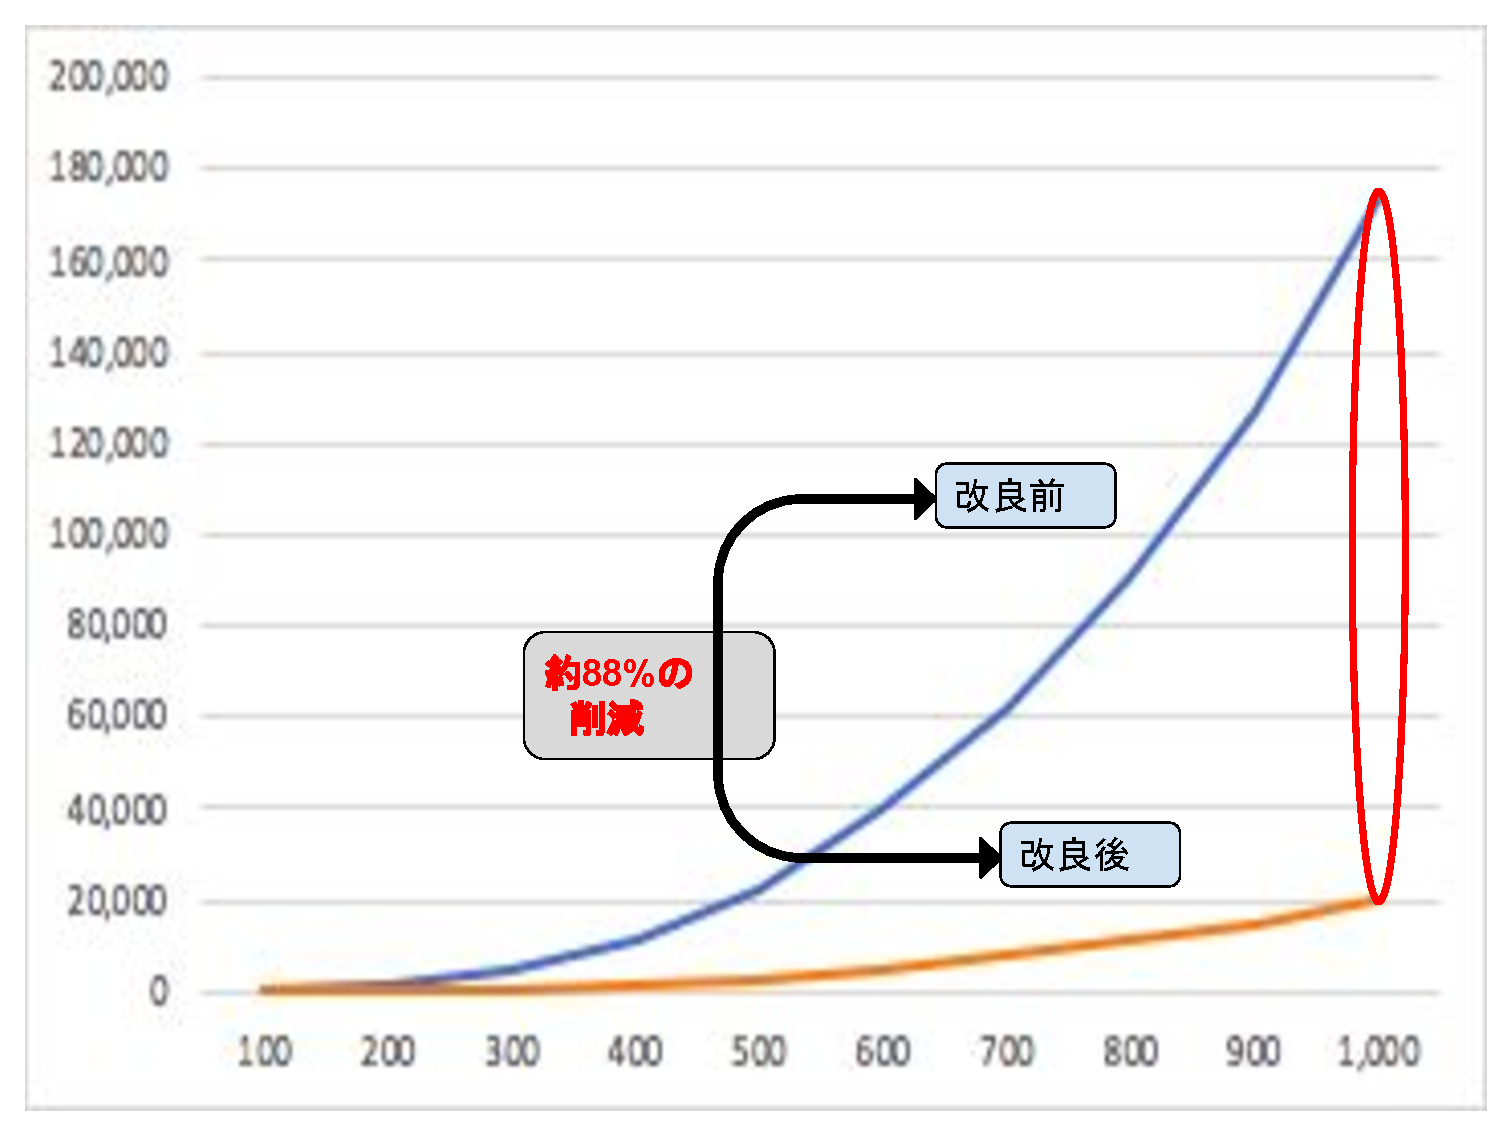
\includegraphics[height=7.0cm , width=15.0cm]{fig/fig13.pdf}
  \caption{多目的最短経路問題に対する提案解法1に用いた,完全多項式時間近似スキームに基づいた
  解の格納方法による計算時間の比較.表  参照}
\end{figure}


\begin{description}
  \item[尺度2:]
  多目的最短経路問題に対する提案解法1に用いた,ラベル付けアルゴリズムに基づいた
  解の格納方法による計算時間の比較.

  図4.11より,頂点数100,重みの範囲100のとき,改良前の計算時間は,1,654,873 ms,改良後の計 算時間は,28 ms であった.
  つまり,ラベル付けアルゴリズムに基づいた解の格納方法の改良により,約99\%の計算時間の削減を可能にした.
  頂点数の増加に伴い,格納方法による改良前と改良後の計算時間の差は拡大している.
  そのため,頂点数をさらに増やすことで削減率も上がると考えられる.

\end{description}

\begin{figure}[htbp]
  \centering
  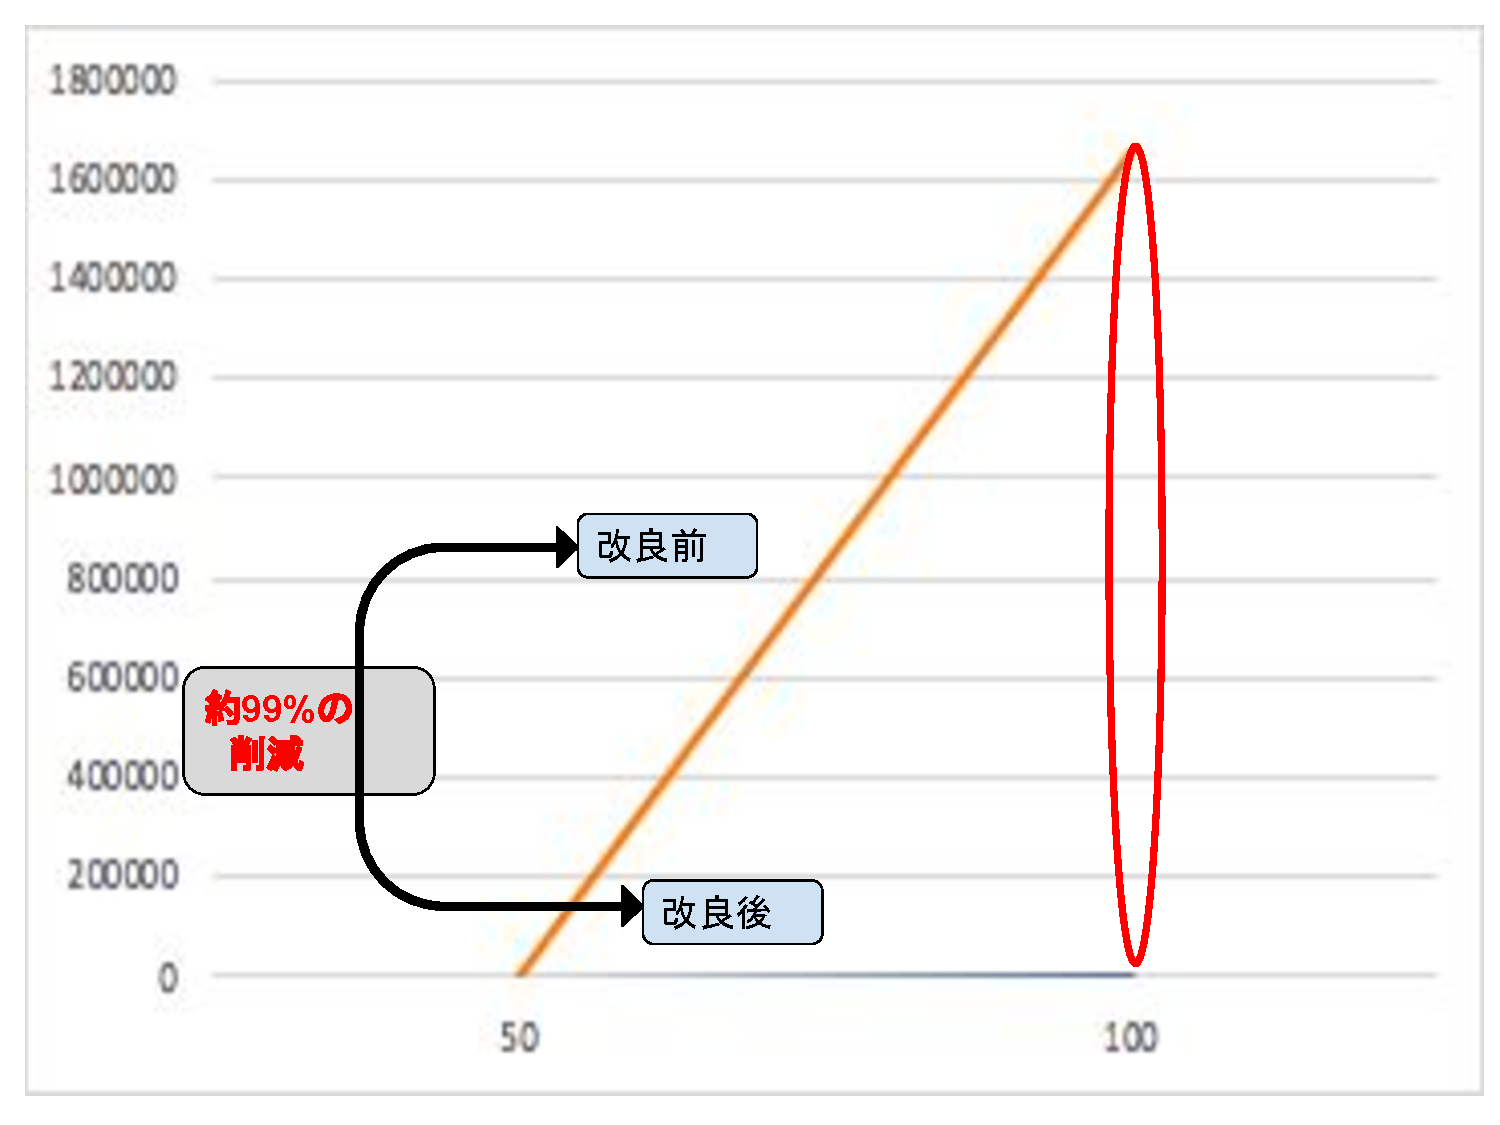
\includegraphics[height=7.0cm , width=15.0cm]{fig/fig14.pdf}
  \caption{多目的最短経路問題に対する提案解法1に用いた,ラベル付けアルゴリズムに基づいた
  解の格納方法による計算時間の比較.表  参照}
\end{figure}


\begin{description}
  \item[尺度3:]
  多目的最短経路問題に対する提案解法2に用いた,動的計画法に基づいた探索順序による計算時間の比較.

  図4.12より,頂点数1000,重みの範囲1000のとき,改良前の計算時間は,14,016 ms,改良後の計 算時間は,8,900 ms であった.
  つまり,探索順序の改良により,約36\%の計算時間の削減を可能にした.
  この結果に対する考察を行う.提案解法2の場合,探索順序を変更することによって無駄な探索を減らし探索にかかる時間を削減しているが,
  探索順序を変更するためにラベルを多く作っているため全体に対する探索の終了後にラベル内の解を移動させる操作が多くなる.
  (提案解法1では,更新対象とするもの$\rightarrow$更新対象としないもの.提案解法2では,更新対象とするもの$\rightarrow$更新対象としないもの,
  次回更新対象とするもの$\rightarrow$更新対象とするもの.)
  ここで,相関係数と計算時間の関係を見ていくと,相関が大きくなるにつれて解の数は少なくなり,計算時間が短くなっている.
  目的関数の相関と解の数の関係より,相関が大きくなるにつれて解の数は少なくなるため削除される解の数も少なくなる.
  削除される解の数が少なくなると提案解法2の優位性が低くなる.
  結果より,無駄な探索をしないことによる時間の削減<
  ラベル内の解を移動させる操作にかかる時間となっていると考えられる.
  頂点数の増加に伴い,格納方法による改良前と改良後の計算時間の差は拡大している.
  そのため,頂点数をさらに増やすことで削減率も上がると考えられる.

\end{description}

\begin{figure}[htbp]
  \centering
  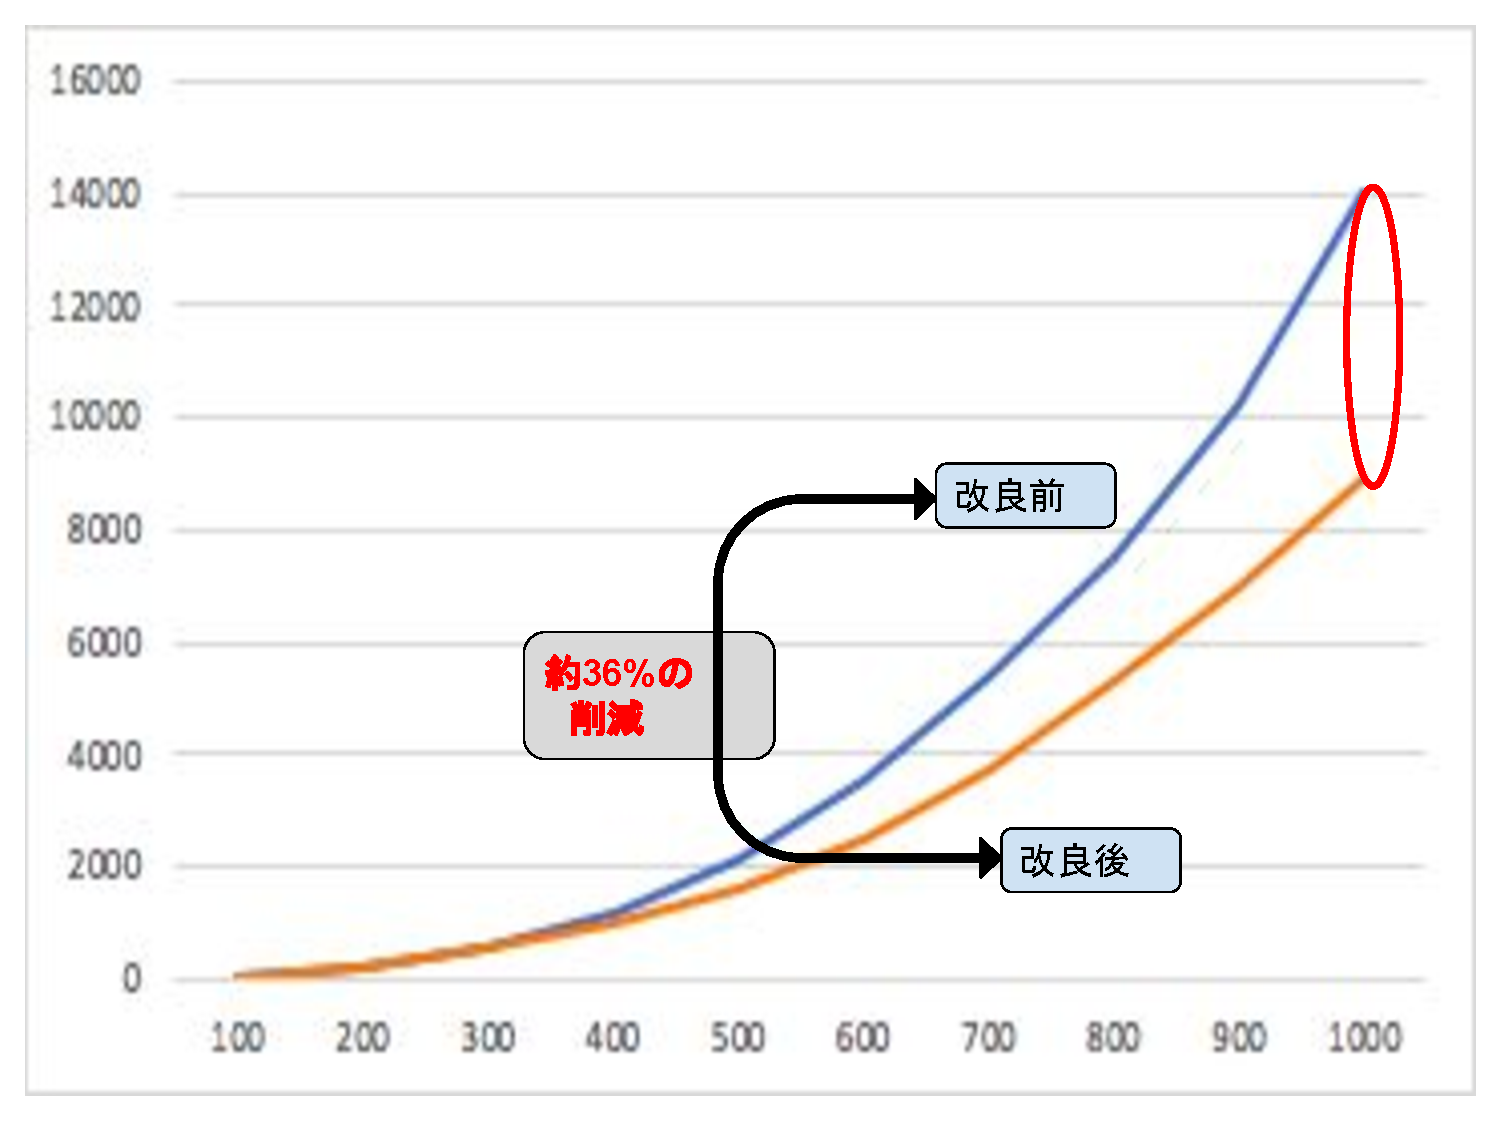
\includegraphics[height=7.0cm , width=15.0cm]{fig/fig15.pdf}
  \caption{多目的最短経路問題に対する提案解法2に用いた,動的計画法に基づいた
  探索順序による計算時間の比較.表  参照}
\end{figure}


\begin{description}
  \item[尺度4:]
  多目的最短経路問題に対する提案解法1と提案解法2において,各目的関数の相関係数による計算時間の比較.

  図4.13より,頂点数1000,重みの範囲1000のとき,目的関数の相関係数の値が約0.90のときに提案解法1の計算時間が
  提案解法2の実装時間より短くなっている.つまり,目的関数の相関係数の値が約0.90のときに計算時間が逆転している.
  この結果に対する考察を行う.提案解法2の場合,探索順序を変更することによって無駄な探索を減らし探索にかかる時間を削減しているが,
  探索順序を変更するためにラベルを多く作っているため全体に対する探索の終了後にラベル内の解を移動させる操作が多くなる.
  (提案解法1では,更新対象とするもの$\rightarrow$更新対象としないもの.提案解法2では,更新対象とするもの$\rightarrow$更新対象としないもの,
  次回更新対象とするもの$\rightarrow$更新対象とするもの.)
  ここで,相関係数と計算時間の関係を見ていくと,相関が大きくなるにつれて解の数は少なくなり,計算時間が短くなっている.
  目的関数の相関と解の数の関係より,相関が大きくなるにつれて解の数は少なくなるため削除される解の数も少なくなる.
  削除される解の数が少なくなると提案解法2の優位性が低くなる.
  結果より,目的関数の相関係数の値が約0.90以上のとき,無駄な探索をしないことによる時間の削減<
  ラベル内の解を移動させる操作にかかる時間となっていると考えられる.
  図4.13は頂点に入ってくる辺の重みベクトルに対しての相関を求めているが,頂点から出ていく辺の重みベクトルに対しての相関
  でも同じことが言える.頂点に入ってくる辺の重みベクトルに対しての相関と頂点から出ていく辺の重みベクトルに対しての相関
  の間には関係が存在しないため,両方の相関が低い場合のみ,無駄な探索をしないことによる時間の削減>
  ラベル内の解を移動させる操作にかかる時間となる.

\end{description}

\begin{figure}[htbp]
  \centering
  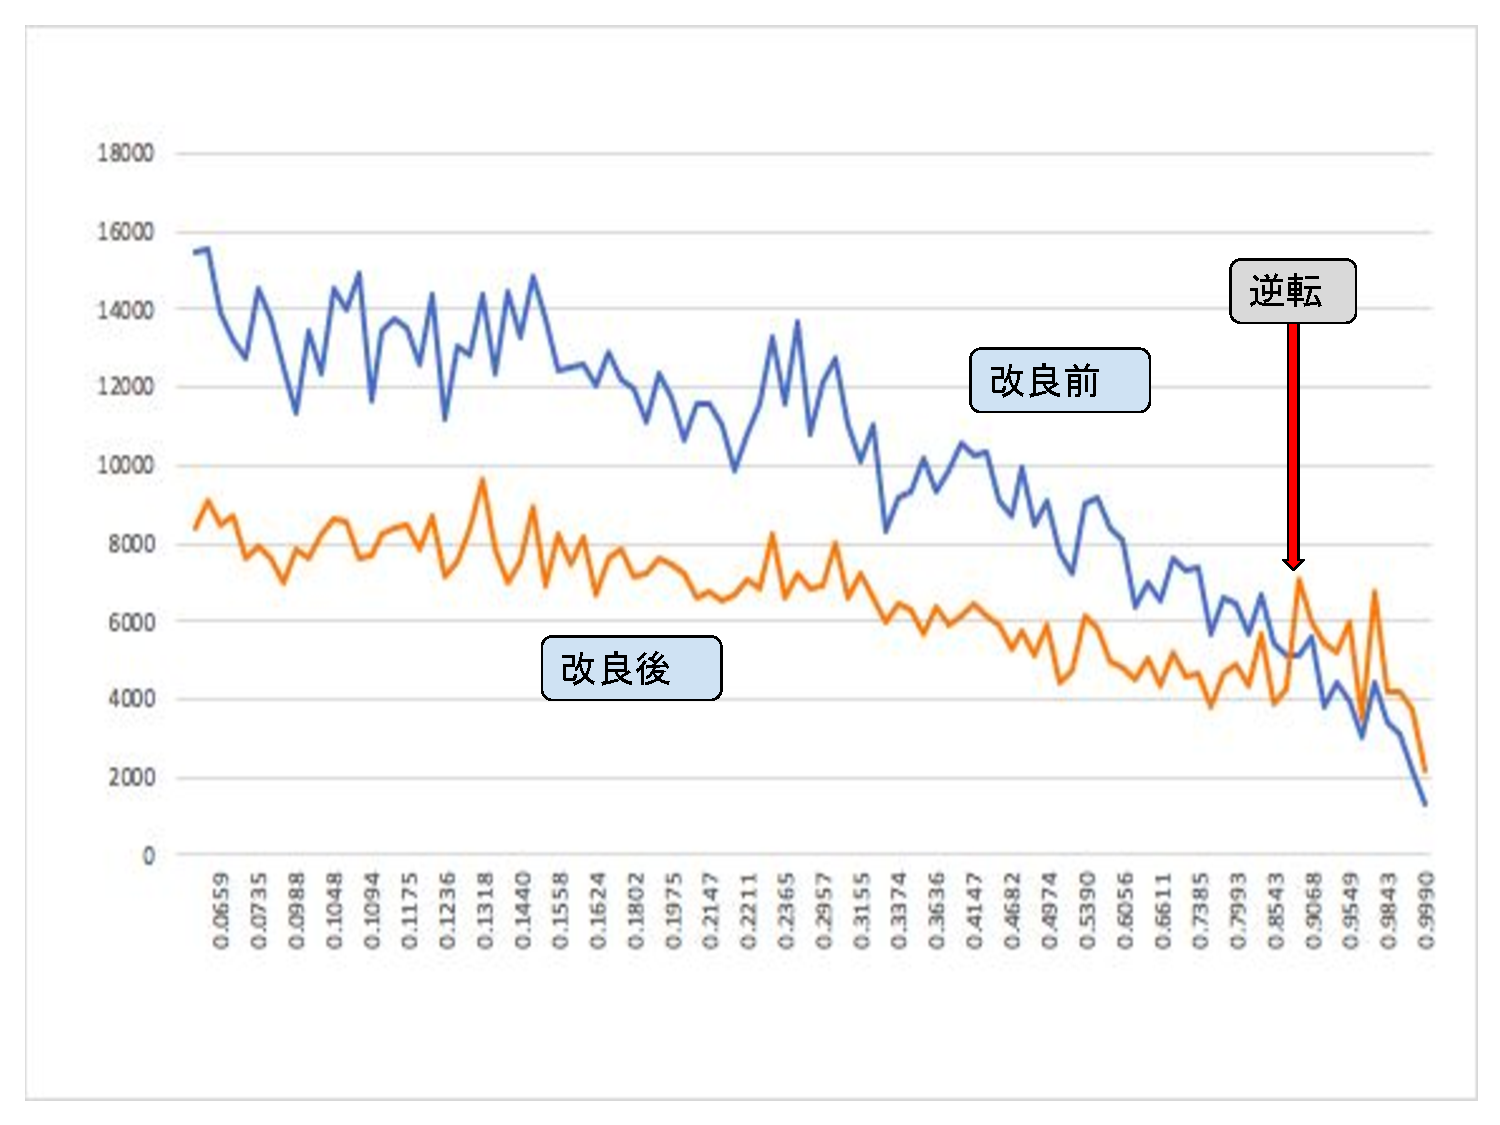
\includegraphics[height=7.0cm , width=15.0cm]{fig/fig18.pdf}
  \caption{多目的最短経路問題に対する提案解法1と提案解法2において,各目的関数の相関係数による計算時間の比較.表  参照}
\end{figure}


\begin{description}
  \item[負の値を考慮した解法の評価と分析]
\end{description}

実数(負の要素を含む)の多目的最短経路問題に対して,本研究で提案した解法の実験的評価を行なった.
評価方法は各インスタンスに対して,本研究で提案する3つの解法により出力された解から得られた平均実装時間
を比較するものである.負のサイクルが存在しない場合を考慮するために非負数の場合も比較する.
また,最大削減率を求めるため,重みの範囲=頂点数,最適化目的の数=3とし,各目的関数間の相関は弱いものとする.
負のサイクルが存在するときの比較のため3つの目的関数のうち1つの目的関数に負のサイクルが存在している.

\begin{description}
  \item[尺度1:]
  負のサイクルが存在しない多目的最短経路問題に対する負の要素を考慮した解法による計算時間の比較.

  頂点数1000,重みの範囲1000のとき,負の閉路を先に検出したときの計算時間は,12,921 ms,探索途中で負の閉路を検出したときの
  計算時間は,12,683 ms,負の閉路検出で得られた解を基に探索したときの計算時間は,28,756 ms であった.
  つまり,負の閉路を先に検出した場合と探索途中で負の閉路を検出した場合の計算時間がもっとも短いということになる.
  この結果に対する考察を行う.負の閉路を先に検出した場合と探索途中で負の閉路を検出した場合,
  負の閉路検出に多少の時間はかかるが探索順序は提案解法2と同じになる.
  しかし,負の閉路検出で得られた解を基に探索した場合の探索順序は提案解法2と異なる.
  これは,探索開始時の更新対象となる解が多く存在しているためである.
  負の閉路検出で得られた解は経由する頂点が複数であるpathであるため,負の閉路検出で得られた解を基にして
  探索したときに得られる解は後に他の解に支配され削除される可能性が高い.そのため,非効率であると考えられる.
  頂点数の増加に伴い,格納方法による改良前と改良後の計算時間の差は拡大している.
  そのため,頂点数をさらに増やすことでそれぞれに対する効率の差が大きくなると考えられる.

\end{description}

\begin{description}
  \item[尺度2:]
  負のサイクルが存在する多目的最短経路問題に対する負の要素を考慮した解法による計算時間の比較.

  % 図より,頂点数1000,重みの範囲1000のとき,負の閉路を先に検出したときの計算時間は,12,921 ms,探索途中で負の閉路を検出したときの
  % 計算時間は,12,683 ms,負の閉路検出で得られた解を基に探索したときの計算時間は,28,756 ms であった.
  % つまり,負の閉路を先に検出した場合と探索途中で負の閉路を検出した場合の計算時間がもっとも短いということになる.
  % この結果に対する考察を行う.負の閉路を先に検出した場合と探索途中で負の閉路を検出した場合,
  % 負の閉路検出に多少の時間はかかるが探索順序は提案解法2と同じになる.
  % しかし,負の閉路検出で得られた解を基に探索した場合の探索順序は提案解法2と異なる.
  % これは,探索開始時の更新対象となる解が多く存在しているためである.
  % 負の閉路検出で得られた解は経由する頂点が複数であるpathであるため,負の閉路検出で得られた解を基にして
  % 探索したときに得られる解は後に他の解に支配され削除される可能性が高い.そのため,非効率であると考えられる.
  % 頂点数の増加に伴い,格納方法による改良前と改良後の計算時間の差は拡大している.
  % そのため,頂点数をさらに増やすことでそれぞれに対する効率の差が大きくなると考えられる.

\end{description}

\begin{description}
  \item[工夫に対する評価と分析]
\end{description}

非負数の多目的最短経路問題に対して,本研究で提案した解法の実験的評価を行なった.
評価方法は各インスタンスに対して,本研究で提案する提案解法により出力された解から得られた平均実装時間と,
実装における工夫を考慮しない提案解法2により出力された解から得られた平均実装時間と比較するものである.
また,最大削減率を求めるため,重みの範囲=頂点数,最適化目的の数=3とし,各目的関数間の相関は弱いものとする.

\begin{description}
  \item[尺度1:]
  多目的最短経路問題に対する提案解法2に用いた,リスト構造による計算時間の比較.

  図より,頂点数500,重みの範囲500のとき,ArrayListを使用したときの計算時間は,2,913 ms,配列を用いた双方向リストの
  計算時間は,2,037 ms,classを用いた双方向リストの計算時間は,1,789 ms であった.
  つまり,classを用いた双方向リストの計算時間がもっとも短いということになる.
  この結果に対する考察を行う.ArrayListを使用した場合,双方向リストは使用できないため解の追加/削除,ラベルからラベルへの
  解の移動にかかる計算時間が長くなるため全体の実装時間が長くなったと考えられる.
  逆に,双方向リストを使用した場合,解の追加/削除,ラベルからラベルへの
  解の移動にかかる計算時間が短くなるため全体の実装時間が短くなったと考えられる.
  classを使用した場合,解が増えるたびに新しい変数を作成するため計算時間がかかる.
  配列を用いた場合,メモリ削減のため空の要素を管理し解の保存場所を決定するため計算時間がかかる.
  解の数が大きくなるほど空の管理は難しくなるため,インスタンスが大きくなるにつれて非効率になると考えられる.
  頂点数の増加に伴い,格納方法による改良前と改良後の計算時間の差は拡大している.
  そのため,頂点数をさらに増やすことでそれぞれに対する効率の差が大きくなると考えられる.

\end{description}

\begin{description}
  \item[尺度2:]
  多目的最短経路問題に対する提案解法2に用いた,更新対象による計算時間の比較.

  図より,頂点数500,重みの範囲500のとき,始点を更新対象としたときの計算時間は,
  終点を更新対象としたときの計算時間は,1,789 ms であった.
  つまり,終点を更新対象としたときの計算時間が始点を更新対象としたときの計算時間より短いということになる.
  この結果に対する考察を行う.
  辺の始点を更新対象とする場合を考える.辺の始点を更新対象としたとき頂点から出ていく辺の向かう先の頂点(辺の終点)は違うため,
  パレート解となるか判断するリストは次に参照するまでの時間が長くなると予想されキャッシュに保存しておくことが難しい.
  反対に辺の終点を更新対象としたとき探索したpathがパレート解となるか判断するリスト
  は辺の終点のリストのためキャッシュに溜め込んでおくことが可能で探索したpathがパレート解となるか判断する
  ための参照時間は短くなると予想される.複数のpathにパレート解となるかの判断が必要で,その度にリストを参照するため
  リストの参照時間が短くなると実装時間も短くなると予想される.
  頂点数の増加に伴い,格納方法による改良前と改良後の計算時間の差は拡大している.
  そのため,頂点数をさらに増やすことでそれぞれに対する効率の差が大きくなると考えられる.

\end{description}

\chapter{結論}

\section{研究成果}

\begin{description}
  \item[成果1:]
  非負数における多目的最短経路問題に対して,
  ベルマンフォード法の探索順序およびデータの格納に改良を加えた解法を提案した.

  完全多項式時間近似スキームに基づいた解法を参考にしたのデータの格納に対して,
  すでに更新されたpathが更新対象とならない格納方法を実装し,計算時間を最大90\%削減した.
  ラベル付けアルゴリズムに基づいた解法を参考にしたのデータの格納に対して,
  比較対象や探索対象となるpathが発見しやすい格納方法を実装し,計算時間を最大99\%削減した.
  更新対象を限定した動的計画法を用いることにより,
  全体のpathに対する更新途中で発見されたpathが更新対象にならないようにすることで,
  経由する頂点数が少ないpathから順に探索されるよう実装をし,計算時間を最大36\%削減した.

  以上の改良より,従来研究のもっとも実装時間の短い解法と比較した結果,
  同じインスタンスに対して計算時間を最大90\%削減した.
\end{description}

\begin{description}
  \item[成果2:]
  各目的関数間の相関係数と問題の難しさを明らかにした.

  各目的関数間の相関係数が大きい,すなわち相関が強いとき支配されて解とならないpathが多く存在し,
  全体のパレート解の数が少なくなることを考え実験的に証明した.また,解の数に応じて問題がより難しくなり
  計算時間が多くかかることを示したため,各目的関数間の相関が弱いとき問題は難しくなる.
  提案した解法は探索順序を変更することで削除される解の数を少なくし計算時間を削減するものだったため,
  各目的関数間の相関により解の数が少なくなると削除される解の数も少なくなるため,各目的関数間の相関
  によって有効な解法になり得ないことを実験的に示した.よって,先の提案解法が有効な解法となる場合がある.

  以上より,頂点数や重みの範囲が同じでも,各目的関数間の相関係数によって解の数や実装時間
  が変化することを実験的に証明し,有効な解法を提案した.
\end{description}

\begin{description}
  \item[成果3:]
  負のサイクルが存在する場合を考慮した解法を提案した.

  多目的最短経路問題において負のサイクルが存在する場合,負のサイクルが存在しない目的関数のみでの
  パレート解と定義し,負のサイクルの検出を行う解法を提案した.
  以上より,多目的最短経路問題における負のサイクルの検出を行うことで負の要素を考慮し,
  扱えるインスタンスの範囲を広げた.
\end{description}

\begin{description}
  \item[まとめ:]
  本研究では最適化目的の数=3である単一始点最短経路問題に対する解法を提案した.
  しかし,最適化目的の数が3より多い場合の検証は行えておらず全点対最短経路問題に対する
  解法は提案できていない.
\end{description}

\section{今後の課題}
以下に,本研究で明らかにできなかった課題を今後の課題としてまとめる.

\begin{description}
  \item[課題1:]
  多目的全点対最短経路問題に対する解法の提案.

  本研究では,1つの始点からその他の頂点への最短経路を求める多目的単一始点最短経路問題
  についての解法を行なった.しかし,最短経路問題には,任意の頂点間の最短経路を求める
  全点対最短経路問題が存在するため多目的最適化問題においても考慮すべきであるが,
  効率的な解法は提案されていない.

\end{description}



\begin{description}
  \item[課題2:]
  インスタンスの大規模化.

  本研究では,1つの計算機での実装を行うための解法を提案したが,1つの計算機での計算には限界がある.
  そこで並列計算手法を考える.複数の計算機を通信を用いて使用することにより,より大規模なインスタンス
  が実装可能になることが考えられる.

\end{description}


\bibliographystyle{splncs03}
\addcontentsline{toc}{chapter}{\bibname}
\bibliography{thesis_nakano}
\appendix


\chapter{多目的最短経路問題に対する解法の実験結果}
% \begin{table}[h]
%   \centering
%   \caption{CI安定集団構造構成の実験結果(94.5万回)}
%   {\small
%   \begin{tabular}{|c|c|c|c|c|} \hline
%     プレイヤー数 & 逸脱回数 & 平均 & 最小逸脱回数 & 最大逸脱回数 \\ \hline
%     n=10  & 2,727,254 & 2.886 & 0 & 12 \\ \hline
%     n=20  & 6,461,477 & 6.838 & 0 & 21 \\ \hline
%     n=30  & 10,224,722 & 10.820 & 0 & 32 \\ \hline
%     n=40  & 13,950,718 & 14.763 & 2 & 41 \\ \hline
%     n=50  & 17,608,330 & 18.633 & 3 & 52 \\ \hline
%     n=60  & 21,209,044 & 22.443 & 5 & 63 \\ \hline
%     n=70  & 24,764,379 & 26.206 & 7 & 67 \\ \hline
%     n=80  & 28,269,979 & 29.915 & 9 & 77 \\ \hline
%     n=90  & 31,734,205 & 33.581 & 10 & 84 \\ \hline
%     n=100 & 35,159,676 & 37.206 & 12 & 91 \\ \hline
%     n=110 & 38,549,466 & 40.793 & 13 & 99 \\ \hline
%     n=120 & 41,919,499 & 44.359 & 13 & 103 \\ \hline
%     n=130 & 45,241,468 & 47,875 & 16 & 105 \\ \hline
%     n=140 & 48,546,345 & 51.372 & 16 & 113 \\ \hline
%     n=150 & 51,829,043 & 54.846 & 20 & 118 \\ \hline
%     n=160 & 55,092,815 & 58.299 & 20 & 125 \\ \hline
%     n=170 & 58,342,060 & 61.738 & 21 & 129 \\ \hline
%     n=180 & 61,571,985 & 65.156 & 25 & 135 \\ \hline
%     n=190 & 64,784,887 & 68.555 & 24 & 137 \\ \hline
%     n=200 & 67,988,416 & 71.945 & 28 & 142 \\ \hline
%     n=210 & 71,168,737 & 75.311 & 27 & 152 \\ \hline
%     n=220 & 74,346,258 & 78.673 & 28 & 152 \\ \hline
%     n=230 & 77,512,643 & 82.024 & 33 & 158 \\ \hline
%     n=240 & 80,662,688 & 85.357 & 34 & 165 \\ \hline
%     n=250 & 83,816,500 & 88.695 & 36 & 170 \\ \hline
%     n=260 & 86,935,408 & 91.995 & 39 & 171 \\ \hline
%     n=270 & 90,072,723 & 95.315 & 41 & 176 \\ \hline
%     n=280 & 93,213,031 & 98.638 & 41 & 183 \\ \hline
%     n=290 & 96,311,780 & 101.917 & 43 & 182 \\ \hline
%     n=300 & 99,428,033 & 105.215 & 43 & 190 \\ \hline
%   \end{tabular}
%   }
% \end{table}
%


\chapter*{謝辞}
本研究を進めるにあたり,指導教員の宋 少秋教授には研究に対する助言や熱心な指導
をしていただきましたことを心から感謝いたします.またゼミや日常で多くの
知識や示唆をいただいた研究室の先輩,
同期の方々に感謝いたします.

\begin{flushright}
  2019年1月31日 \氏名
\end{flushright}
\endmatter % 削除しないように!
\end{document}
